\documentclass[landscape]{article}
\usepackage[ngerman]{babel}
\usepackage[utf8]{inputenc}
\usepackage{multicol}
\usepackage{calc}
\usepackage{ifthen}
\usepackage[landscape]{geometry}
\usepackage{amsmath,amsthm,amsfonts,amssymb}
\usepackage{color,graphicx,overpic}
\usepackage{listings}
\usepackage[compact]{titlesec} %less space for headers
\usepackage{mdwlist} %less space for lists
\usepackage{pdflscape}
\usepackage{verbatim}
\usepackage[hidelinks,pdfencoding=auto]{hyperref}
\usepackage{fancyhdr}
\usepackage{lastpage}
\pagestyle{fancy}
\fancyhf{}
\fancyhead[L]{Computergrafik}
\fancyfoot[L]{\thepage/\pageref{LastPage}}
\renewcommand{\headrulewidth}{0pt} %obere Trennlinie
\renewcommand{\footrulewidth}{0pt} %untere Trennlinie

\pdfinfo{
    /Title (Computergrafik - Cheatsheet)
    /Creator (TeX)
    /Producer (pdfTeX 1.40.0)
    /Author (Robert Jeutter)
    /Subject ()
}

% This sets page margins to .5 inch if using letter paper, and to 1cm
% if using A4 paper. (This probably isn't strictly necessary.)
% If using another size paper, use default 1cm margins.
\ifthenelse{\lengthtest { \paperwidth = 11in}}
    { \geometry{top=.5in,left=.5in,right=.5in,bottom=.5in} }
    {\ifthenelse{ \lengthtest{ \paperwidth = 297mm}}
    {\geometry{top=1.3cm,left=1cm,right=1cm,bottom=1.2cm} }
    {\geometry{top=1.3cm,left=1cm,right=1cm,bottom=1.2cm} }
    }

% Redefine section commands to use less space
\makeatletter
\renewcommand{\section}{\@startsection{section}{1}{0mm}%
                                {-1ex plus -.5ex minus -.2ex}%
                                {0.5ex plus .2ex}%x
                                {\normalfont\large\bfseries}}
\renewcommand{\subsection}{\@startsection{subsection}{2}{0mm}%
                                {-1explus -.5ex minus -.2ex}%
                                {0.5ex plus .2ex}%
                                {\normalfont\normalsize\bfseries}}
\renewcommand{\subsubsection}{\@startsection{subsubsection}{3}{0mm}%
                                {-1ex plus -.5ex minus -.2ex}%
                                {1ex plus .2ex}%
                                {\normalfont\small\bfseries}}
\makeatother

% Don't print section numbers
\setcounter{secnumdepth}{0}

\setlength{\parindent}{0pt}
\setlength{\parskip}{0pt plus 0.5ex}    
% compress space
\setlength\abovedisplayskip{0pt}
\setlength{\parskip}{0pt}
\setlength{\parsep}{0pt}
\setlength{\topskip}{0pt}
\setlength{\topsep}{0pt}
\setlength{\partopsep}{0pt}
\linespread{0.5}
\titlespacing{\section}{0pt}{*0}{*0}
\titlespacing{\subsection}{0pt}{*0}{*0}
\titlespacing{\subsubsection}{0pt}{*0}{*0}

\begin{document}
\raggedright
\scriptsize
\begin{multicols}{3}
  
  % multicol parameters
  % These lengths are set only within the two main columns
  %\setlength{\columnseprule}{0.25pt}
  \setlength{\premulticols}{1pt}
  \setlength{\postmulticols}{1pt}
  \setlength{\multicolsep}{1pt}
  \setlength{\columnsep}{2pt}
  
  \section{Mathematik Grundlagen}
  \begin{description*}
    \item[Vektor] $\vec{x}=(x_1,x_2,...,x_n)$
    \begin{description*}
      \item[Ortsvektor] $(x,y,z,1)^T$
      \item[Richtungsvektor] $(x,y,z,0)^T$
    \end{description*}
    \item[Multiplikation] $\alpha * \vec{x} = (\alpha *x_1, \alpha *x_2,...)$
    \item[Addition] $\vec{x}+\vec{r}=(x_1+r_1, x_2+r_2,...)$
    \item[Linearkombination] $\vec{o} = (\alpha * \vec{p})+(\beta *\vec{q})+(\gamma * \vec{r})$
    \item[Länge] $\vec{p}=(x,y,z): |\vec{p}|=\sqrt{x^2+y^2+z^2}$
    \item[Skalarprodukt] $\vec{x}*\vec{r}=\sum_{i=0}^{n-1} x_i*r_i$
    \item[Winkel] $\vec{a}*\vec{b}=|\vec{a}|*|\vec{b}|*cos(\phi)$ mit $cos(\phi)=\frac{\vec{a}*\vec{b}}{|\vec{a}|*|\vec{b}|}$
    \item[Vektorprodukt] $\vec{a}\times\vec{b} = \begin{pmatrix} a_y b_z - a_z b_y \\ a_z b_x - a_x b_z \\ a_x b_y - a_y b_x \end{pmatrix}$
    \item[Ebenen] $p=\vec{q}+\alpha*\vec{r}+\beta * \vec{s}$
    \item[Dreieck] $\vec{A}+\alpha*(B-A)+\beta*(C-A)$
    \item[Strahlensatz] $y'_P = \frac{y_P*z_e}{z_P}$
    \item[Kugeloberfläche] $A_k = 4\pi r^2$
  \end{description*}
  
  \subsection{2D Transformation}
  \begin{description*}
    \item[Translation] um den Vektor $\vec{t}$
    \item[Skalierung] Stauchung oder Streckung
    \item[Spiegelung]
    \begin{itemize*}
      \item an x-Achse $S=\begin{pmatrix} 1 & 0 \\ 0 & -1 \end{pmatrix}$
      \item an y-Achse $S=\begin{pmatrix} -1 & 0 \\ 0 & 1 \end{pmatrix}$
      \item am Ursprung $S=\begin{pmatrix} -1 & 0 \\ 0 & -1 \end{pmatrix}$
    \end{itemize*}
    \item[Scherung] $S=\begin{pmatrix} 1 & S_x \\ S_y & 1 \end{pmatrix}$
    \item[Rotation mit Polarkoordinaten] $P'=(r,\phi+\theta)$; $\binom{x'}{y'}=\begin{pmatrix} cos(\theta) & -sin(\theta) \\ sin(\theta) & cos(\theta)\end{pmatrix}*\binom{x}{y}$
    \item[Koordinatentransformation] $P\rightarrow P'$ \newline $P' =T*P = \begin{pmatrix} x_x & x_y\\ y_x & y_y \end{pmatrix} * \binom{P_x}{P_y}$
  \end{description*}
  
  Kartesische Koordinaten bezeichnen die Koordinaten direkt\\
  Homogene Koordinaten besitzen ein zusätzliches Gewicht w
  
  \paragraph{Homogene Vektorräume}
  kartesischer Vektor $(\frac{x}{w},\frac{y}{w})$ oft $w=1$ gewählt (1=Punkt, 0=Richtung)
  
  \begin{description*}
    \item[Skalierung, Projektion, Spiegelung] $\begin{pmatrix} F_x & 0 & 0 \\ 0 & F_y & 0 \\ 0 & 0 & 1 \end{pmatrix} * \begin{pmatrix} x \\ y \\ 1 \end{pmatrix} = \begin{pmatrix} F_x*x \\ F_y*y \\ 1 \end{pmatrix}$
    
    $F_x,F_y>0$, uniform bei $F_X=F_y$\newline    
    $F_x=0$/$F_y=0$:Projektion auf y/x-Achse\newline    
    $F_x=-1$/$F_y=-1$ Spiegelung an y/x-Achse\newline    
    $F_x=F_y=-1$Spiegelung am Ursprung
    
    \item[Scherung] $\begin{pmatrix} 1 & a & 0 \\ 0 & 1 & 0 \\ 0 & 0 & 1 \end{pmatrix} * \begin{pmatrix} x \\ y \\ w \end{pmatrix} = \begin{pmatrix} x+a*y \\ y \\ w \end{pmatrix}$
    \item[Rotation] $R_\theta *P= \begin{pmatrix}cos(\theta) & -sin(\theta) & 0 \\ sin(\theta) & cos(\theta) & 0 \\ 0 & 0 & 1 \end{pmatrix} * \begin{pmatrix}x & y & 1 \end{pmatrix} = \begin{pmatrix} x cos(\theta) - y sind(\theta)\\ x sin(\theta)+y cos(\theta)\\ 1 \end{pmatrix}$
  \end{description*}
  
  \paragraph{Invertierung}
  \begin{description*}
    \item[Transformation]  $T_{\Delta x, \Delta y}^{-1} = T_{-\Delta x, -\Delta y}$
    \item[Skalierung] $S_{F_x, F_y}^{-1}=S_{\frac{1}{F_x},\frac{1}{F_y}}=\begin{pmatrix} \frac{1}{F_x} &0&0\\ 0&\frac{1}{F_y}&0\\ 0&0&1 \end{pmatrix}$
    \item[Rotation] $R_{-\theta} = \begin{pmatrix} cos(\theta) & sin(\theta) & 0 \\ -sin(\theta) & cos(\theta) & 0 \\ 0 & 0 & 1 \end{pmatrix} = R_{\theta}^{T}$
    \item[Verknüpfungen] $(A*B*C)^{-1}=C^{-1}*B^{-1}*A^{-1}$
  \end{description*}
  
  \paragraph{Affine Abbildung}
  $$\begin{pmatrix}a_1 & b_1 & c_1\\a_2 &b_2 & c_2\\ 0&0&1\end{pmatrix}*\begin{pmatrix} x_1\\y_1\\1\end{pmatrix}= \begin{pmatrix}x_1'\\y_1'\\1 \end{pmatrix}$$
  \begin{itemize*}
    \item die letzte Zeile der affinen Matrix bleibt immer 0,0,1
    \item paralleles bleibt bei affinen Abbildungen stets parallel
  \end{itemize*}
  
  \subsection{Homogene Transformation in 3D}
  $(a,b,c,d)$ wobei $(a,b,c)=(nx,ny,nz)$ und $d$ der Abstand der Ebene zum Ursprung
  \begin{itemize*}
    \item Ebene definiert durch 3 Punkte
    $$\begin{pmatrix}
        x_1 & x_2 & x_3 & 0 \\
        y_1 & y_2 & y_3 & 0 \\ 
        z_1 & z_2 & z_3 & 0 \\
        1   & 1   & 1   & 1
      \end{pmatrix}$$
    \item Translation um Vektor $(\Delta x, \Delta y,\Delta z)$
    $$\begin{pmatrix}
        1 & 0 & 0 & \Delta x \\
        0 & 1 & 0 & \Delta y \\ 
        0 & 0 & 1 & \Delta z \\
        0 & 0 & 0 & 1
      \end{pmatrix}$$
    \item Skalierung um Faktor $F_x,F_y,F_z$
    $$\begin{pmatrix}
        F_y & 0   & 0   & 0 \\
        0   & F_y & 0   & 0 \\ 
        0   & 0   & F_z & 0 \\
        0   & 0   & 0   & 1
      \end{pmatrix}$$
    \item Rotation um die x-Achse
    $$\begin{pmatrix}
        1 & 0           & 0            & 0 \\
        0 & cos(\theta) & -sin(\theta) & 0 \\ 
        0 & sin(\theta) & cos(\theta)  & 0 \\
        0 & 0           & 0            & 1
      \end{pmatrix}$$
    \item Rotation um die y-Achse
    $$\begin{pmatrix}
        cos(\theta)  & 0 & sin(\theta) & 0 \\
        0            & 1 & 0           & 0 \\ 
        -sin(\theta) & 0 & cos(\theta) & 0 \\
        0            & 0 & 0           & 1
      \end{pmatrix}$$
    \item Rotation um z-Achse
    $$\begin{pmatrix}
        cos(\theta) & -sin(\theta) & 0 & 0 \\
        sin(\theta) & \cos(\theta) & 0 & 0 \\ 
        0           & 0            & 1 & 0 \\
        0           & 0            & 0 & 1
      \end{pmatrix}$$
    \item Berechnung
    $$\begin{pmatrix} a& b& c& 0\\ d& e& f& 0\\ g& h& i& 0\\ 0& 0& 0& 1\end{pmatrix}
      * \begin{pmatrix} x \\ y \\ z \\ 0 \end{pmatrix}
      = \begin{pmatrix} ax+bx+cz \\ dx+ey+fz \\ gx+hy+iz \end{pmatrix}$$
  \end{itemize*}
  
  \paragraph{Kameratransformation}
  Kamera ist definiert durch
  \begin{itemize*}
    \item Lage des Augpunktes E (in Weltkoordinaten)
    \item Blickrichtung D
    \item Oben-Vektor U ('view up vector', senkrecht zu D)
  \end{itemize*}
  Transformation durch
  \begin{itemize*}
    \item Ursprung in Augpunkt
    \item negative z-Achse in Blickrichtung
    \item y-Achse nach oben
  \end{itemize*}
  
  \subsection{Projektion}
  \paragraph{Orthogonale Projektion}
  \begin{itemize*}
    \item Projektionsebene ist parallel zur XY Ebene
    \item Projektionsrichtung stets parallel zur z-Achse (rechtwinklig zur Projektionsebene)
    \item z Koordinaten werden auf gleichen Wert gesetzten
  \end{itemize*}
  
  \paragraph{Schiefwinklige Parallelprojektion}
  \begin{itemize*}
    \item typische Parallelprojektion mit 2 Parametern
    \item Projektionsebene ist parallel zur XY Ebene
    \item Projektionsrichtung hat zwei Freiheitsgrade und ist typischerweise nicht orthogonal zur Projektionsebene
    \item Projektionsrichtung (Schiefe) ist über 2 Winkel parametrisierbar
    \item Herleitung $P=\begin{pmatrix}
        1 & 0 & -cos(\alpha)*f & 0  \\
        0 & 1 & -sin(\alpha)*f & 0  \\
        0 & 0 & 0              & 0  \\
        0 & 0 & 0              & 1 
      \end{pmatrix}$
    \item es gilt: $x'=x-cos(\alpha)*f*z$ und $y'=y-sin(\alpha)*f*z$
  \end{itemize*}
  
  \paragraph{Zentralperspektive}
  \begin{itemize*}
    \item entspricht einer Lochkamera bzw etwa dem 'einäugigen' Sehen
    \item Augpunkt im Ursprung des Kamerakoordinatensystems
    \item Projektionsfläche ist eine Ebene parallel zu XY Ebene
    \item Eigenschaften
    \begin{itemize*}
      \item perspektivische Verkürzung
      \item parallele Linien des Objekts fluchten oft in einen Fluchtpunkt
    \end{itemize*}
    \item Strahlensatz: $\frac{y_p}{d}=\frac{y}{z}\Rightarrow y_p=\frac{d*y}{z}$
  \end{itemize*}
  $$\begin{pmatrix} d&0&0&0\\ 0&d&0&0 \\ 0&0&0&1 \\ 0&0&1&0 \end{pmatrix} * \begin{pmatrix}x\\y\\z\\1\end{pmatrix} = \begin{pmatrix} d*x\\ d*y\\ 1 \\ z \end{pmatrix} \rightarrow \begin{pmatrix} \frac{d*x}{z} \\ \frac{d*y}{z} \\ \frac{1}{z} \end{pmatrix}$$
  
  \paragraph{Fluchtpunkte}
  \begin{itemize*}
    \item Wird aus einer Richtung r und dem Augpunkt eine Gerade definiert, dann schneidet diese Gerade die Projektionsfläche im Fluchtpunkt für die Richtung r
    \item hat ein Modell parallele Kanten oder parallele Striche in Texturen, dann ergibt sich für jede solche Richtung r in der Abbildung ein Fluchtpunkt, auf den diese parallelen Kanten/Striche hinzu zu laufen scheinen
    \item es gibt jedoch Ausnahmen, bei denen Paralleles in der Abbildung Parallel bleibt (z.B. horizontale Kanten bei Schwellen)
    \item Da es beliebig viele Richtungen geben kann, sind auch beliebig viele Fluchtpunkte in einem Bild möglich
    \item Rotationen können Fluchtpunkte ändern, Translationen jedoch nicht
    \item Ermittlung: aus Richtung r und Augpunkt eine Gerade, dann schneidet diese Gerade die Projektionsfläche im Fliuchtpunkt für die Richtung r.
  \end{itemize*}
  
\end{multicols}
\newpage
\begin{multicols}{3}
  \section{Modellierung}
  
  \paragraph{Boundary Representation (B-Rep)}
  \begin{itemize*}
    \item Beschreibung durch die begrenzende Oberflächen
    \item Darstellungsform eines Flächen- oder Volumenmodells
    \item Definition des Ojekts über vef-Graph (vertex, edge, face)
    \begin{itemize*}
      \item Knotenliste: beinhaltet Koordinatenpunkt
      \item Kantenliste: pro Kante zwei Punkte referenziert
      \item Flächenliste: pro Fläche die Reihenfolge der Kanten
    \end{itemize*}
    \item Szene: dreidimensionale Beschreibung von Objekten, Lichtquellen und Materialeigenschaften mit Betrachter
    \item Szenegraph: Gruppierung der Objekte in einer Szene
  \end{itemize*}
  
  \paragraph{Vertex Shader}
  \begin{itemize*}
    \item verarbeitet alle Eckpunkte (Vertices) mit Shader
    \item ermöglicht eine Beeinflussung der Objektform
    \item Transformation der 3D Position auf 2D Koordinaten
    \item Input: Vertices relevanter Objekte und gewünschte Transformation
    \item Output: projizierte 2D Koordinaten mit Tiefeninformationen
  \end{itemize*}
  
  \paragraph{Model View Projection}
  \begin{itemize*}
    \item Gegeben
    \begin{itemize*}
      \item Modell als Vertices mit kartesischen 3D Koordinaten
      \item betrachtende Kamera (3D Position, Ausrichtung)
    \end{itemize*}
    \item Umsetzung
    \begin{enumerate*}
      \item $M=T*R*S$ Transformation von Modellraum in Weltkoordinaten (Model)
      \item $V=T_V^{-1}*R_V^{-1}$ Transformation in Kameraraum (View)
      \item Projektion auf Kamerabildebene und Umrechnung in Bildraum (Projektion)
    \end{enumerate*}
    \item Ergebnis
    \begin{itemize*}
      \item MVP-Matrix $P*V*M=MVP_{Matrix}$
      \item Bildraumprojektion des Modells $p'_m=P*V*M*p_m$
    \end{itemize*}
  \end{itemize*}
  
  \subsection{Effiziente geometrische Datenstrukturen}
  \paragraph{Bintree}
  \begin{itemize*}
    \item logarithmische Komplexität pro Zugriff möglich
    \item Gefahr: lineare Komplexität, wenn nicht balanciert
    \item typisch Teilung in Mitte (bisektion)
    \item Bereiche mit homogenem Inhalt werden nicht unterteilt
    \item Komprimierungseffekt
  \end{itemize*}
  \begin{center}
    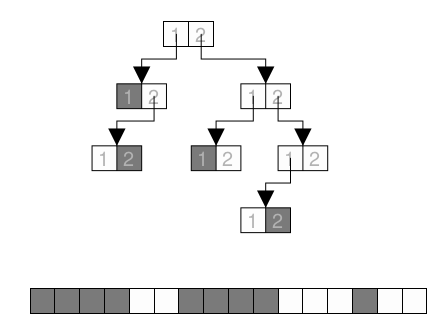
\includegraphics[width=.3 \linewidth]{Assets/Computergrafik_Bintrees}
    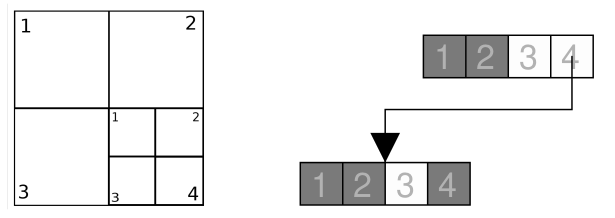
\includegraphics[width=.5 \linewidth]{Assets/Computergrafik_Quadtree}
  \end{center}
  
  \paragraph{Quadtree}
  \begin{itemize*}
    \item eine Fläche wird in vier gleichgroße Quadranten unterteilt
    \item Fläche wird unterteilt bis homogenität
    \item Komprimierung, da nur strukturierte Bereiche unterteilt
  \end{itemize*}
  
  \paragraph{Octree}
  \begin{itemize*}
    \item Objekte in hierarchische Strukturen einsortiert
    \item jeder Knoten hat 0 oder 8 Kindknoten (8 Unterbereiche)
    \item beschleunigte räumliche Suche
    \item Zeitaufwand Tiefe des Baumes $O(\log n)$
  \end{itemize*}
  
  \paragraph{KD Tree}
  \begin{itemize*}
    \item mehrdimensionaler binärer Baum (k-dimensional)
    \item Teilung nicht zwangsläufig mittig $\rightarrow$ an Daten angepasst
    \item pro Hierarchiestufe stets wechsel der Teilungsrichtung
    \item Median-Cut Strategie: Teilung in zwei gleichgroße Hälften
    \begin{itemize*}
      \item Baum garantiert balanciert und Tiefe minimal
      \item $O(\log n)$ Verhalten garantiert
      \item Probleme bei lokalen Häufungen (Cluster)
      \item unnötige Unterteilung weit weg (Artefakt)
    \end{itemize*}
    \item Middlecut-Strategie:
    \begin{itemize*}
      \item nicht balanciert
      \item keine Unterteilung weit weg vom Cluster
    \end{itemize*}
    \item ein Octree lässt sich auf kd-Baum abbilden, beide Baumarten haben daher vergleichbare Eigenschaften
  \end{itemize*}
  \begin{center}
    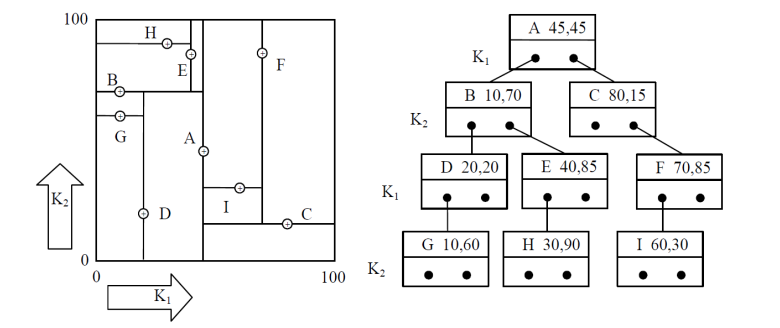
\includegraphics[width=.5 \linewidth]{Assets/Computergrafik_KD-tree}
  \end{center}
  
  \paragraph{BSP Tree}
  \begin{itemize*}
    \item Verallgemeinerung des kd-Baums
    \item Trennebenen nicht nur achsenparallel
    \item Unterteilung adaptiv an Modellflächen angepasst
    \item Trennebenen können weiter weg liegende Objekte schneiden
    \item führt bei konvexen Polyedern zu entarteten Bäumen
  \end{itemize*}
  
  \paragraph{Hüllkörper Hierarchie}
  \begin{description*}
    \item[AABB] (Axis-Aligned-Bounding-Box) sehr einfache Abfrage (nur ein Vergleich $<$ pro Koordinatenrichtung) einfach zu erstellen (min, max), dafür nicht optimale Packungsdichte bei schräger Lage der Objekte
    \item[OBB] (Oriented Bounding Boxes) passen sich besser der räumlichen Ausrichtungen an, lassen sich auch leicht transformieren. Jedoch schwieriger zu erstellen (Wahl der Richtung), komplexere Überlappungsberechnung. Typischerweise weniger tief, weniger räumliche Abfragen dafür wesentlich mehr Berechnungsaufwand pro Rekursionsstufe.
    \item[KDOP] (k-dim. Discretly Oriented Polytopes) Polyeder mit festen vorgegebenen Richtungen. Eigenschaften zwischen AABB und OBB. Bessere Raumausnützung als AABB, weniger Transformationene als OBB.
    \item[BS] (Bounding Spheres) Schnelle 3D Überlappungstest (Abstand der Mittelpunkte $<$ Summe der Radien). Langgezogene Objekte können mit mehreren Hüllkugeln begrenzt werden um besseren Füllgrad zu erreichen. BS sind, bis auf die Lage der Kugelmittelpunkte, invariant gegenüber Rotation (geeignet für Kollisionserkennung bewegter Objekte).
    \item[weitere Anwendungsfälle] Kollisionserkennung in Computeranmiation. Reduktion der potenziellen Kollisionspaare durch räumliche Trennung. Beschleunigung des Echtzeitrenderings großer Datenmengen. Reduktion des Aufwands durch Culling (Weglassen)
  \end{description*}
  
  \paragraph{Ray Picking mit KD Baum}
  \begin{itemize*}
    \item Vorverarbeitung von Objekten im kd-Baum $O(n \log n)$
    \item Strahl/Objektschnitt: als rekursive Suche im kd-Baum
    \item $treeIntersect$: Findet Schnittpunkt des Strahls mit den im Baum gespeicherten Dreiecken
    \item $triangleIntersect$: Findet Schnittpunkt des Strahles mit Menge von Dreiecken in node
    \item $subdivide$: Findet rekursiv den nächstgelegenen Schnittpunkt (kleinstes t) des Strahls im Parameterbereich 
  \end{itemize*}
  
  \paragraph{Aufwandsabschätzung bzgl Dreiecksanzahl}
  \begin{itemize*}
    \item konvexes Objekt: Komplexität einer räumlichen Punktsuche, also zur Untersuchung einer Baumzelle $O(\log n)$
    \item Polygonnebel: viele kleine Dreiecke im Such-Volumen
    \item alle Zellen enthalten konstante kleine Anzahl von Dreiecken $\rightarrow$ Aufwand proportional zur Anzahl durchlaufener Baumzellen
    \item Anzahl dieser Zellen ist proportional zur Länge des Strahls durchs Volumen, da der 1. Schnitt sehr wahrscheinlich mitten im Volumen oder gar nicht stattfindet $\rightarrow$ Anzahl ist proportional zur Seitenlänge des Suchvolumens
    \item bei n Dreiecken im Suchvolumen ist die Anzahl t der zu untersuchenden Zellen also ca $t=O(\sqrt{n})$ $\rightarrow$ Suchaufwand pro Strahl folglich $O(\sqrt{n} \log (n))$
  \end{itemize*}
  
  \paragraph{Aufwandsabschätzung in fps}
  \begin{itemize*}
    \item absoluter Gesamtaufwand zum Raytracing einer Szene ist proportional zur Anzahl der Strahlen
    \item rekursives RT (Reflexion, Brechung, Schattenstrahlen etc) entsprechend mehr Strahlen, d.h. weniger Performance
    \item Parallelisierung einfach möglich $\rightarrow$ früher CPU, heute GPU
  \end{itemize*}
  
  \paragraph*{Heurisitk zur Unterteilung}
  \begin{itemize*}
    \item Surface Area Heuristic (SAH):
    \begin{itemize*}
      \item Strahl $i$ trifft Zelle $j$ mit Wahrscheinlichkeit $P(i,j)$, zudem sei $n_j$ die Anzahl Dreiecke in Zelle $j$
      \item Aufwand für Raytracing pro Zelle proportional zur Baumtiefe und Anzahl der dortigen Dreiecke $n_j$;$\rightarrow$ Gesamtaufwand für Strahl $i$ sei  $\sum(P(i,j)*n_j)$
    \end{itemize*}
    \item große Zellen mit wenigen Dreiecken senken Gesamtaufwand
    \item $P(i,j)$ ist proportional zur Oberfläche einer Zelle
    \item SAH optimiert das Produkt der Zellgröße mal Anzahl Dreiecke im Teilbaum. Für den kD-Baum in Richtung k: $D_k = D_{k_{links}} + D_{k_{rechts}}$
    \item bei ungleicher Verteilung der Dreiecke enthalten große Zellen wenige oder keine Dreiecke und Baum ist nicht balanciert $\rightarrow$ implizite Abtrennung des Clusters vom Rest des Baums (vgl. Middle-Cut-Strategie)
  \end{itemize*}
  
  \paragraph{Behandlung ausgedehnter Objekte}
  \begin{itemize*}
    \item Punkte haben keine Ausdehnung und können an einem eindeutigen Ort im kD-Baum abgelegt sein
    \item Ausgedehnte Objekte können räumlich mehrere Blatt- Zellen überlappen. Diese Objekte müssen dann in mehreren Blattzellen einsortiert werden
  \end{itemize*}
  \begin{enumerate*}
    \item Auftrennung von Objekten, d.h. Objekte müssen an der Zellgrenze aufgeteilt werden. Einsortierung der Teilobjekte in passende Zellen. Geht gut für Dreiecke
    \item Keine Unterscheidung zwischen Blattknoten und inneren Knoten. In diesem Ansatz werden Objekte soweit oben im Baum einsortiert, dass sie keine Zellgrenze schneiden. Nachteil: auch relativ kleine Objekte müssen in große Zellen einsortiert werden, wenn sie deren Unterteilungsgrenze schneiden
    \item Loose Octree: die Zellen des Octrees werden so vergrößert, dass sie mit ihren direkten Nachbarn in jeder Richtung um 50\% überlappen. Objekte, die im einfachen Octree aufgrund ihrer Größe Grenzen schneiden würden, können im Loose Octree in den Zwischenknoten gespeichert werden. Ein Objekt mit Durchmesser bis zu $\frac{D}{2^L}$ kann auf der Ebene L abgelegt werden. Eine Suche im Loose Octree muss daher außer der direkt betroffenen Zelle auch die überlappenden direkten Nachbarn berücksichtigen. Dadurch vergrößert sich der Aufwand einer Suche um einen konstantne Faktor. Beachte: Die asymptotosche Komplexität (O-Notation) ist dadurch nicht beeinflusst.
  \end{enumerate*}
  
\end{multicols}
\newpage
\begin{multicols}{3}
  \section{Rastergrafik}
  
  \subsection{ Midpoint Algorithmus}
  \begin{itemize*}
    \item Effizient durch Ganzzahlen, Vermeiden von $*,/$, \item Nutzung inkrementeller Arbeitsweise
    \item Bresenham-Algorithmus: Mittelpunkt M; jeweils aktuellen Punkt P, der rechts von im liegende E (east) und der rechts oben liegende NE (north-east) benannt.
    \item die Linie wird als Funktion repräsentiert: $y=\frac{\delta y}{\delta x}*x+B$
    \item implizierte Form: $d: F(x,y)=\delta y*x-\delta x*y+B*\delta x = 0$
    \item für Punkte auf der Linie wird $F(x,y)=0$
    \item für Punkte unterhalb der Linie wird $F(x,y)>0$
    \item für Punkte oberhalb der Linie wird $F(x,y)<0$
    \item Herleitung: Steigung der Linie m ($-1<m<1$), Punkt vertikal zwischen zwei Pixeln E und NE. Falls $F(x_p + 1, y_p+\frac{1}{2})>0$ wird das nächste Pixel NE, andernfalls E
    \item Insgesamt acht verschiedene Fälle nach Oktanten
  \end{itemize*}
  \begin{center}
    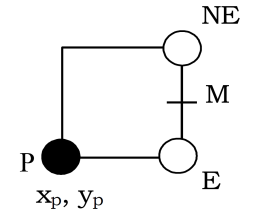
\includegraphics[width=.2\linewidth]{Assets/Computergrafik_Midpoint}
  \end{center}
  
  \paragraph{Anti Aliasing}
  \begin{center}
    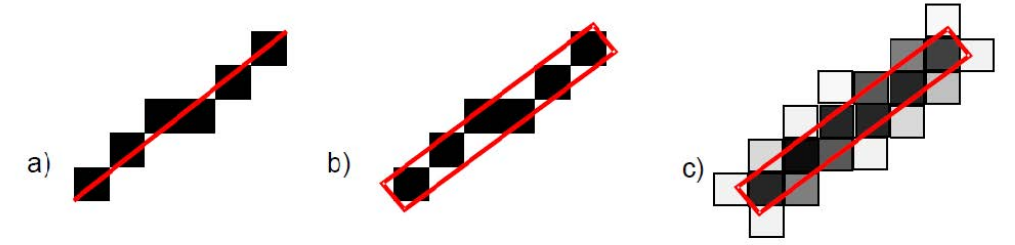
\includegraphics[width=.5\linewidth]{Assets/Computergrafik_Antialiasing}
  \end{center}
  \begin{itemize*}
    \item Treppenstufeneffekt bei gerasterten Linien
    \item Auflösungsvermögen des Auges für Punkte sei e. Strukturen wie Linien werden durch Mittelwertbildung (Fitting) vom Auge viel genauer als e lokalisiert. Eine Stufe wird umso eher erkannt, je länger die angrenzenden Segmente sind.
    \begin{itemize*}
      \item Statt Linie wird Rechteck mit Breite eines Pixels betrachtet
      \item Graustufen darunter liegender Pixelflächen entsprechen jew. Überdeckungsgrad
    \end{itemize*}
    \item Praktische vereinfachte/effiziente Umsetzung
    \begin{itemize*}
      \item Rasterkonvertierung der Linie bei doppelter örtlicher Auflösung (Supersampling)
      \item Replizieren der Linie (vertikal und/oder horizontal) um Linienbreite näherungsweise zu erhalten
      \item Bestimmmung des Überdeckungsgrades pro Pixel in der ursprünglichen Auflösung (Downsampling)
      \item Bestimmung des Farbwertes entsprechend des Überdeckungsgrades
    \end{itemize*}
    \item Ideales Antialiasing: wegen beliebig komplexen Geometrie allgemein sehr hoher Aufwand
    \item Ansatz für eine 'reale Lösung'
    \begin{itemize*}
      \item ideale Berechnung von Farbwerten irrelevant
      \item Ansätze mit gut abschätzbarem/konstanten Aufwand
      \item Verwendung mehrerer Samples pro Pixel
    \end{itemize*}
    \item A.A. erhöht empfundene räumlich Auflösung
  \end{itemize*}
  
  \paragraph{Supersampling + Downsampling}
  \begin{itemize*}
    \item Grafik in höherer Auflösung gerendert (z.B. 4-fach) und aus Samples ein Farbwert gemittelt
    \item Ohne A.A. pro Pixel eine Sampleposition$\Rightarrow$ gefärbt o. nicht
    \item Es gibt immer eine Abstufung mehr als Subpixel pro Pixel
    \item Bei vier Subpixeln können 0-4 Subpixel im Pixel gesetzt sein, d.h. 5 Intensitäten von 0\%, 25\%, 50\%, 75\% oder 100\%
    \item bei Formabhängigkeit gibt es nur eine Zwischenstufe nach Phasenlage $\rightarrow$ Kante 'pumpt' bei Objektbewegung.
    \item $Pixelfarbe= g*Linienfarbe+(1-g)*Hintergrundfarbe$
  \end{itemize*}
  
  \paragraph{Supersampling + Rotated Grids}
  \begin{itemize*}
    \item minderung der Formabhängigkeit
    \item kleine Winkel führen zu langen Stufen der Polygonkante
    \item bessere Verhältnisse der Grauabstufung für flache Winkel, wenn ordered-grid statt rotated-grid verwendet wird
    \item Rotated grids bei anderen Winkeln etwas schlechter als ordered grid
    \item gute Grauabstufung bei sehr flachen Kanten
    \item optimaler Winkel bei ca. 20-30° z.B. $arctan(0.5) \approx 26,6^{\circ}$
    \item sehr dünne Linien bleiben auch bei Bewegung zusammenhängend (Vermeidung von 'Line Popping')
  \end{itemize*}
  
  \paragraph{Supersampling + Multisampling}
  \begin{itemize*}
    \item ein Superbackpuffer (großem Buffer)
    \begin{itemize*}
      \item Nachteil (bei rotated grid): Anpassung der Rasterkonvertierung an verschobene Positionen
      \item Vorteil: Verwendung von mehr Texturinformation (Textur wird subpixelgerecht eingetragen)
    \end{itemize*}
    \item mehrere Multisamplebuffer (mehrere kleinere Buffer)
    \begin{itemize*}
      \item Mehrfachrendering in normaler Größe mit versetzter Geometrie (Vertexverschiebung pro Sub-Bild)
      \item Vorteil: keine Veränderung im Rendering
      \item Nachteil: nur ein Texturwert pro Makro-/Sub-Pixel
    \end{itemize*}
    \item Gezielter Ressourceneinsatz durch Kantenglättung
    \begin{itemize*} 
      \item Effizienzsteigerung durch Beschränkung auf reine Kantenglättung möglich
      \item Aliasing bei Mustern in Texturen schon beim Auslesen der Werte aus Pixeltextur unterdrückbar
      \item Kantenpixel bekannt als separate Linien oder Berandung von Polygonen/Dreiecken
    \end{itemize*}
    \item adaptives Samplen: statt feste Anzahl nach dem Bedarf
  \end{itemize*}
  
  \paragraph{Quincunx Verfahren}
  \begin{itemize*}
    \item 2x Multisampling mit rotated grid; Informationszuwachs durch doppelte Anzahl von Samples
    \item Information für Kantenglättung beruht auf 2 Subpixeln
    \item Entspricht zusätzlicher Tiefpass-Überfilterung. Durch Unschärfe sehen Polygonkanten glatter aus.
    \item Harte Kanten nicht mehr möglich; Rand 'Zappeln' reduziert
    \item Aber: Texturinformation, von 2$>$Subpixeln, verschmiert
  \end{itemize*}
  
  \paragraph{Pseudozufälliges Supersampling}
  \begin{itemize*}
    \item Kombination: Supersampling, Multisampling und Quincunx
    \item bei Überwindung der Grenzen für Füllrate und Bandbreite überwiegen Vorteile des Supersamplings
    \item Ordered/rotated grid weisen nach Strukturklassen Vor-/Nachteile auf. Verbleibende Artefakte wiederholen sich bei großen Flächen - oft als störend empfunden
    \item pszufällige Auswahl von Abtastmustern für Supersampling
    \item nachträgliche Abminderung regelmäßiger Strukturen durch vorsichtiges Verrauschen (Rauschfilter)
    \item entfernungsabhängiges Antialiasing
    \item pseudozufällig
    \begin{itemize*}
      \item Samples können nur an n vordefinierten Positionen stattfinden (Sample-Positionsmuster)
      \item Je nach Methode werden daraus m Positionen für das Samplen zufällig ausgewählt (beachte: $m < n$)
      \item Anzahl der Muster als kombinatorisches Problem: m aus n (ohne Wiederholungen)
    \end{itemize*}
  \end{itemize*}
  
  \paragraph{Downsampling}
  Mittelwertbildung: lineare Filterung (2x - AA), bilineare Filterung (4x - AA). Gleichgültig ob ordered/rotated grid. 
  Beim pseudozufälligen Supersampling ist entsprechend der 'frei gewählten' Positionen der 'Subpixel' zu modifizieren (z.B. Gewichte nach Abstand der Abfragepositionen zur Makropixelposition)
  
  \subsection{Polygonfüllalgorithmus}
  \begin{itemize*}
    \item Ansatz
    \begin{itemize*}
      \item finde die Pixel innerhalb des Polygons
      \item weise ihnen Farbe zu
      \item dabei zeilenweises Vorgehen pro Rasterlinie
      \item schneide die Polygonkante mit der aktuellen Bildzeile
      \item füge Schnittpunkt $x_s$ in eine Liste ein
      \item sortiere Schnittpunkte der Bildzeile in x-Richtung
      \item Paritätsregel: fülle die Pixel jeweils nur zwischen ungeraden und nächstem geraden Schnittpunkt
    \end{itemize*}
    \item Allgemeine Sicht auf die Strategie: Ein Pixel wird mit der Farbe des Polygons gefüllt, das sich rechts von ihm befindet. Sollte dort eine Kante sein, so wird die Farbe des oberen Polygons verwendet.
    \item Effiziente Ermittlung der Schnittpunkte
    \begin{itemize*}
      \item Polygonkanten von unten nach oben bearbeitet
      \item horizontale Polygonkanten nicht bearbeiten $\rightarrow m\not=0$
      \item $d_y = y_1 - y_0$ ist stets positiv (auch nie 0)
      \item $d_x = x_1 - x_0$ kann positiv und negativ sein
      \item damit können 4 Bereiche unterschieden werden
      \item Berechnung von x bzw y: 
      \begin{itemize*}
        \item $y=y_0+m(x-x_0)= y_0+\frac{y_1-y_0}{x_1-x_0}(x-x_0)$,
        \item $x=x_0+\frac{1}{m}(y-y_0)= x_0+\frac{x_1-x_0}{y_1-y_0}(y-y_0)$
      \end{itemize*}
      \item x-/y-Werte noch nicht ganzzahlig
      \item Die Rundung kann inkrementell ermittelt werden
      \item Die Rundungsregel für Bruchwerte hängt davon ab, ob es eine linke oder rechte Kante ist. Links wird z.B. aufgerundet
    \end{itemize*}
    \item Edge-Tabelle
    \begin{itemize*}
      \item Verkettete Liste/Array für nicht-horizontalen Kanten
      \item Sortierung nach Scan-Line, wo Kanten beginnen
      \item In Scan-Line wieder Liste mit z.B. $x_0, y_1$, Zähler
    \end{itemize*}
    \item Active-Edge-Tabelle
    \begin{itemize*}
      \item speichert Kanten die gegenwärtige Scan-Linie schneiden
      \item Liste hat die gleiche Struktur wie eine Zeile der ET
      \item Kanten gelöscht wenn oberes Ende der Kante erreicht
    \end{itemize*}
    \item Scan Convert Polygon: Es existiert immer eine gerade Anzahl Kanten. Viele Grafikbibliotheken beschränkt auf konvexe Polygone. Nichtkonvexe Polygone müssen vorher in konvexe Komponenten zerlegt werden.
    \item Bemerkungen zur Effizienz: Polygon belegt meist mehr Pixel als es Eckpunkte/Kanten besitzt. Deshalb sind effiziente per-Pixel-Operationen wichtig. Der Rechenaufwand sollte vermieden werden (fallende Priorität) für: pro Pixel (sehr häufig auszuführen), pro Rasterzeile, pro Kante (möglichst viel vorberechnen)
  \end{itemize*}
  
  \paragraph{Füllmuster}
  \begin{itemize*}
    \item Füllen eines Polygons mit Pattern statt Farbwert
    \item benutze dazu BITMAPs
    \item 2-dimensionales Array
    \item besteht aus M Spalten und N Zeilen
    \item $BITMAP = ARRAY [0... (M-1), 0...(N-1)]$
  \end{itemize*}
  
  \paragraph{Dithering - Floyd-Steinberg-Algorithmus}
  \begin{itemize*}
    \item Ersetzen 'genauer' Farbwerte durch grobe Quantisierung
    \item Durchlaufen aller Pixel beginnend links oben
    \item pro Pixel P die beste Ersetzung in Tabelle finden \& setzen
    \item verursachte Fehler $\delta$ nach Schema auf unbearbeitete Nachbarpixel verteilen
    \item bei kleinen Bildern mit hoher Auflösung kaum erkennbar
    \item erhöht Farbauflösung $\rightarrow$ Verringert räumlichen Auflösung
    \item komplementär zu A.A.
  \end{itemize*}
  
\end{multicols}
\newpage
\begin{multicols}{3}
  \section{Farbräume}
  
  \subsection{Farbwahrnehmung - Phänonmenologie}
  \begin{itemize*}
    \item Hell- und Farbempfinden als Sinneseindruck beschrieben
    \item Tageslicht als weiß/grau mit unterschiedlichen Helligkeiten aber farblos empfunden
    \item Abwesenheit von Licht wird als schwarz empfunden
    \item Regenbogen bunt mit verschiedenen Farbtönen empfunden
  \end{itemize*}
  
  \begin{description*}
    \item[Farbton] (Hue)
    \begin{itemize*}
      \item Farbpalette aus Abstufung grober Farbtöne 
      \item direkt nebeneinander liegende Farben im Farbspektrum werden als ähnlich empfunden
      \item Farbwerte lassen sich ordnen
      \item als bunt empfunden (voll gesättigte Farben im Gegensatz zu Grautönen)
      \begin{center}
        
\includegraphics[width=.4\linewidth]{Assets/Computergrafik_Farbton}
      \end{center}
    \end{itemize*}
    \item[Farbsättigung] (Saturation)
    \begin{itemize*}
      \item Stufen zwischen Bunt und Grau
      \item Pastelltöne sind weniger bunt aber nicht farblos
      \item Grauton (keine Farbwerte unterscheidbar)
      \item jedem Farbton können Abstufungen bis Grau zugeordnet werden
      \begin{center}
        \includegraphics[width=.4\linewidth]{Assets/Computergrafik_Farbsättigung}
      \end{center}
    \end{itemize*}
    \item[Helligkeitsstufen] (Lightness/Brightness/Value/Intensity)
    \begin{itemize*}
      \item unterschiedliche Helligkeitsabstufungen bis Schwarz
      \item im Schwarzen sind keine Farbtöne mehr unterscheidbar
      \begin{center}
        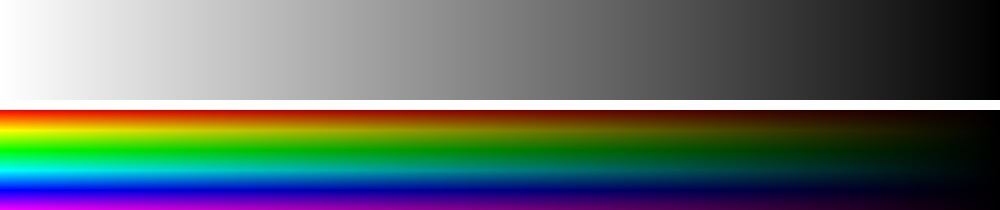
\includegraphics[width=.4\linewidth]{Assets/Computergrafik_Helligkeitsstufen}
      \end{center}
    \end{itemize*}
  \end{description*}
  
  \subsection{Modell der Farben}
  \paragraph{DIN 5033}
  Farbe ist die Empfindung eines dem Auge strukturlos erscheinenden Teils eines Gesichtsfeldes, durch die sich dieser Teil bei einäugiger Beobachtung mit unbewegtem Auge von einem gleichzeitig gesehenem, ebenfalls strukturlos angrenzendem Bezirk allein unterscheidet.
  
  \paragraph{HSL Farbraum (bzw HSB, HSV, HSI)}
  \begin{itemize*}
    \item Dimension des Farbtons wiederholt sich periodisch
    \item Darstellung als Winkelkoordinate eines Polarkoordinaten-Systems in der HS-Ebene oder dreidimensional als Zylinderkoordinaten HSL darstellt.
    \item Darstellungsformen nicht fest vorgeschrieben. Eine Darstellung als (Doppel)-Kegel oder sechseitige (Doppel-) Pyramide ist ebenso möglich
    \item Der HSL Farbraum entspricht grob unserer Farbwahrnehmung. Daher geeignet zur intuitiven und qualitativen Einstellung von Farben in Illustrationsgrafiken
    \item Relative Skala 0-255
    \item Quantisierbarkeit der Farben und Helligkeit
    \item Bezug zur Physik des Lichtes (Energie, Spektrum)
  \end{itemize*}
  
  \paragraph{RGB Farbraum}
  \begin{itemize*}
    \item Hypothese, dass Farbsehen auf drei Arten von Sinneszellen beruht (rot, grün, blau) (Young)
    \item Farbwahrnehmungen durch drei beliebige, linear unabhängige Größen darstellbar (Graßmann)
    \item Mit Grundfarben Rot, Grün und Blau können weitere Farben additiv gemischt werden
    \item Bestimmen der Anteile der Mischfarben
    \begin{itemize*}
      \item Empfindlichkeitskurven R,G,B und zugehörige Lichtquellen r,g,b
      \item alle 3 Lichtquellen zusammen ergeben weis wahrgenommenes Licht: $r=g=b=1$
      \item damit 3d-Farbraum (RGB-Farbraum) aufspannen
      \item Lage einer monochromatischen Lichtwelle: $x(\lambda_0)=p*r+\gamma*g+\beta*b$
      \item Achtung: hängt von Wellenlängen der verwendeten Grundfarben r,g,b (Primärvalenzen) ab.
    \end{itemize*}
    \item Beispiel für Reizung durch monochromatisches Licht (Laser):
    \begin{itemize*}
      \item $r=0,2R(\lambda)$
      \item $y=0,5R(\lambda)+0,3G(\lambda)$
      \item $g=0,2R(\lambda)+0,5G(\lambda)$
      \item $b=0,02B(\lambda)$
    \end{itemize*}
    \item Intensität: $I=\frac{R+G+B}{3}$
    \item Innere Farbmischung: mischen direkt aus Grundfarben
    \item Äußere Farbmischung: hinzufügen von Grundfarben zu bestehender Mischung
  \end{itemize*}
  
  Farberzeugung durch Mischung: $$y=1,9r + 0,6g =0,5R(\lambda)+0,3G(\lambda)$$
  
  Idee:
  \begin{itemize*}
    \item drei linear-unabhängige Größen benötigt, zur Beschreibung und (technischen) Reproduktion der Farbempfindung
    \item zunächst werden folgende Werte gewertet
    \begin{itemize*}
      \item die additive Mischung als Reproduktionsmethode
      \item drei Primärfarben Rot, Grün, Blau
      \item drei linear unabhängige Größen spannen stets einen 3D Raum auf
    \end{itemize*}
    \item die RGB Werte werden den drei ortogonalen Achsen dieses Raumes zugeordnet
  \end{itemize*}
  
  Darstellung des RGB Farbraums:
  \begin{itemize*}
    \item alle technisch/additiv erzeugbaren Farben liegen innerhalb eines Würfels
    \item Im Koordinatenursprung befindet sich Schwarz
    \item auf der Raumdiagonalen liegen dazwischen die Graustufen
  \end{itemize*}
  
  RGB Farbtafel:\\
  Alle Farben gleicher Buntheit führen zum gleichen Farbort, der durch die Farbwertanteile r,g,b beschrieben wird:
  $$r=\frac{R}{R+G+B}, g=\frac{G}{R+G+B}, b=\frac{B}{R+G+B} \leftrightarrow r+g+b=1$$
  
  Aus dem rechten Teil der Gleichung folgt mit $b=1-r-g$, dass sich die Buntheit allein durch r und g darstellen lässt (entspricht $R^2$).  
  
  \subsection{CIE System}
  \begin{minipage}[b]{0.25\textwidth}
    Um eine Relation zwischen der menschlichen Farbwahrnehmung und den physikalischen Ursachen des Farbreizes herzustellen, wurde das CIE-Normvalenzsystem definiert. Es stellt die Gesammtheit der wahrnehmbaren Farben dar.
  \end{minipage}
  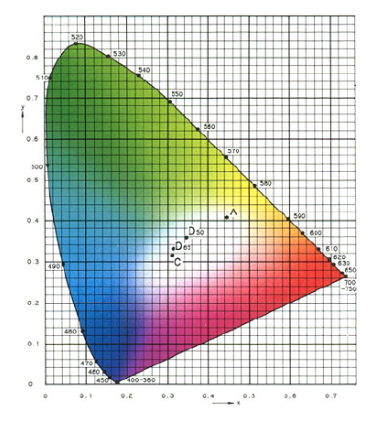
\includegraphics[width=0.15\linewidth]{Assets/Computergrafik_CIE}
  
  \subsubsection{Farbkörperunterschiede}
  Es finden sich Unterschiede welche Farbbereiche nach dem CIE Normalvalenzsystem von den jeweiligen Systemen dargestellt werden können:
  \begin{itemize*}
    \item menschliche Farbwahrnehmung ca. 2-6 Mio Farben
    \item Monitor ca. 1/3 davon. Bei Monitoren wird die additive Farbmischung verwendet, da die einzelnen Lichtquellen aufsummiert werden.
    \item Druckprozess deutlich weniger Farben. Es werden einzelne Farbschichten auf Papier gedruckt und das resultierende Bild wird über subtraktive Farbmischung bestimmt
  \end{itemize*}
  
  \subsubsection{Subtraktive Farbmischung}
  Je nachdem welche Farbe ein Material hat, werden entsprechende Farbanteile absorbiert oder reflektiert. Eine gelbe Oberfläche sieht gelb aus, da sie das Blau aus weißem Licht absorbiert, aber Rot und Grün reflektiert.
  
  Achtung: Dies gilt nur für die Bestrahlung mit weißem Licht. Wird beispielsweise ein gelbes Blatt mit blauem Licht bestrahlt, dann wirkt es schwarz, da das blaue Licht vom gelben Blatt absorbiert wird.
  
  \subsubsection{Umwandlung}
  Von einem Farbort im XYZ-System $F_P=(X Y Z)^T$ in das equivalente CIE Diagramm $F'_P=(X' Y')^T$ durch $$F'_P=\begin{pmatrix}X' \\ Y'\end{pmatrix} = \begin{pmatrix} \frac{X}{X+Y+Z} \\ \frac{Y}{X+Y+Z}\end{pmatrix}$$
  
  \begin{tabular}{l | c | c}
    Farbraum               & gerätespezifisch & gleichabständig \\\hline
    RGB                    & ja               & nein            \\
    CMY                    & ja               & nein            \\
    HSI                    & ja               & nein            \\
    HLS                    & ja               & nein            \\
    XYZ (CIE)              & nein             & nein            \\
    $L*a*b*$ ($CIE_{Lab}$) & nein             & ja              \\
  \end{tabular}
  
\end{multicols}
\newpage
\begin{multicols}{3}
  \section{Licht \& Reflexion}
  \begin{description*}
    \item[Licht] Teil der elektromagnetischen Strahlung
    \item[Photon] Elementarteilchen der elektromagnetischen Wechselwirkung
    \item[Radiometrie] Messung elektromagnetischer Strahlung
    \item[Photometrie] Messverfahren im Wellenlängenbereich
    \item[Strahlungsäquivalent] $K =\frac{\phi_v}{\phi_e}$
    \item[Lumen] 1 Lumen ist der Lichtstrom einer 1,464 mW starken 555-nm-Lichtquelle mit 100\% Lichtausbeute
    \item[Raumwinkel] $\Omega = \frac{Flaeche}{Radius}= \frac{A}{r^2} [sr]$
  \end{description*}
  
  \subsection{Radiometrie (energetisch "$_e$")}
  \begin{description*}
    \item[Q] Strahlungsenergie $Q = \#Photonen * Photonenenergie [J]$
    \item[$\Phi$] Strahlungsleistung $\Phi = \frac{Q}{t} [W]$
    \item[I] Strahlstärke $I = \frac{\Phi}{\Omega} [\frac{w}{sr}]$
    \item[E] Bestrahlungsstärke $E = \frac{\Phi}{A_i} [\frac{W}{m^2}]$
    \item[L] Strahldichte $L = \frac{I}{A'_r} = \frac{\Phi}{cos(\phi * A_r * \Omega)}$
  \end{description*}
  
  \subsection{Photometrie (visuell "$_v$")}
  \begin{description*}
    \item[Q] Lichtmenge $lm * s$
    \item[$\Phi$] Lichtstrom $[Lumen]$
    \item[I] Lichtstärke $[Candela]$ cd   
    \item[E] Beleuchtungsstärke $\frac{lm}{m^2}=I_{in}\cos(\Phi) [Lux]$
    \item[L] Leuchtdichte $\frac{cd}{m^2}$
  \end{description*}
  
  \subsection{Lichtquellen}
  \begin{description}
    \item[Ambient] Licht strahlt gleichmäßig aus jeder beliebigen Richtung
    \item[Parallel] Licht strahlt in gleichmäßigen, parallelen Strahlen aus einer festgelegtenRichtung
    \item[Punkt] Licht  wird  gleichmäßig  in  alle  Richtungen  abgestrahlt
    \item[Spot] Licht wird in den Halbraum abgestrahlt, wobei das meiste Licht in eineVorzugsrichtung abgegeben wird
  \end{description}
  \begin{center}
    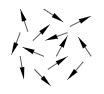
\includegraphics[width=0.15\linewidth]{Assets/Computergrafik_ambientes-licht}
    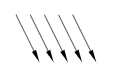
\includegraphics[width=0.15\linewidth]{Assets/Computergrafik_paralleles-licht}
    
\includegraphics[width=0.15\linewidth]{Assets/Computergrafik_punkt-licht}
    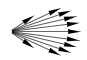
\includegraphics[width=0.15\linewidth]{Assets/Computergrafik_spot-licht}
  \end{center}
  
  \paragraph{Räumliche Ausbreitung}
  Flächen Energieübertragung
  \begin{itemize*}
    \item der Abstand zwischen den beiden Flächen beträgt r
    \item die Flächen stehen nicht notwendigerweise senkrecht zur Ausbreitungsrichtung des Lichts
    \item abstrahlende und empfangende Fläche jeweils in Ausbreitungsrichtung mit projizierten Flächen $A'_r$ und $A'_i$.
    \item Punktlichtquellen von der abstrahlenden Fläche $A_r$, welche ihre Strahlungsleistung in den Raumwinkel $\Omega$ abgeben
    \item $\Omega$ ist somit die in Abstrahlrichtung reduzierte Fläche $A'_i$ , projiziert auf die Einheitskugel: $\Omega=A'_i \backslash r^2$
    \item Die übertragene Energie nimmt quadratisch zu r ab
  \end{itemize*}
  
  \paragraph{Reflexion}
  Nach Auftreffen auf einer opaken Oberfläche wird Strahlung spektral unterschiedlich stark und geometrisch auf unterschiedliche Weise reflektiert. 
  Fälle der Reflexion:
  \begin{itemize*}
    \item spekulär (spiegelnde) Reflexion (Einfallsw.=Ausfallswinkel)
    \item Diffuse Reflexion
    \item Diffus-gerichtete Reflexion
  \end{itemize*}
  \begin{center}
    \includegraphics[width=0.3\linewidth]{Assets/Computergrafik_spekuläre-reflexion}
    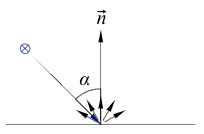
\includegraphics[width=0.3\linewidth]{Assets/Computergrafik_diffuse-reflexion}
    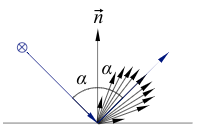
\includegraphics[width=0.3\linewidth]{Assets/Computergrafik_diffus-gerichtete-reflexion}
  \end{center}
  
  \paragraph{Diffuse Reflexion}
  Eingestrahlte Strahlstärke verteilt sich durch Projektion auf größere Fläche. Die Bestrahlungsstärke ist dadurch proportional zum Vergrößerungsfaktor der Fläche abgeschwächt.
  In Richtung Betrachter reflektierte Strahlstärke $I_{out}$ Aufgrund von Interferenz phasengleicher Lichtstrahlen $\rightarrow$ Projektion auf Normalenrichtung $I_{out}= E_{refl} * \cos(\phi)$
  \begin{itemize*}
    \item Senkrecht zur Oberfläche: Maximale Kohärenz (Addition)
    \item Parallel zur Oberfläche: Keine Kohärenz (Auslöschung)
  \end{itemize*}
  
  $$\frac{A_r}{A'_r}=\frac{1}{\cos(\phi)} \rightarrow L=\frac{I_{out}}{\cos(\phi)}=I_{refl}$$
  Ein Betrachter mit flachem Blickwinkel sieht Licht aus größerer Fläche $A_r$ durch Kombination dieser Effekte, kürzt sich der Einfluss des Betrachterwinkels $\cos(\phi)$ weg und es bleibt nur der Einfluss des Lichteinfallswinkels übrig: Strahldichte des reflektierten Lichtes: $L=I_{in}*k_d(\lambda)*\cos(\phi)$
  
  \paragraph{Spekuläre Reflexion}
  (gestreut spiegelnd)
  \begin{itemize*}
    \item Speckles bzw. Facetten sind einzeln jeweils 'ideal'
    \item spiegelnd: $\text{Einfallswinkel } \phi = \neg \text{Ausfallswinkel} = -\phi$
    \item Microfacettenausrichtung weichen von Gesamtflächennormalen ab
    \item dadurch Streuung des Lichts (Keule) um den Winkel $\theta$ der idealen Spiegelung herum
    \item Je größer der Winkel $\theta$ zwischen idealer Spiegelrichtung und Richtung zum Betrachter, desto schwächer ist die Reflexion
    \item Modellierung meist per $\cos^k(\theta)$ (Phong-Modell)
  \end{itemize*}
  
  Gestreute Spiegelung im Phong Modell mit $L=I*k_s*\cos^k(\theta)$
  \begin{itemize*}
    \item glänzende Fläche: großer Exponent k; kleine Streuung $\epsilon$
    \item matte Fläche: kleiner Exponent k; große Streuung $\epsilon$
  \end{itemize*}
  
  Für Energieerhaltung zusätzlicher Normierungsfaktor benötigt:
  \begin{itemize*}
    \item physikalisch nicht korrekt:  $L=I*k_s*\cos^k(\theta)$
    \item gebräuchliche Normierung $L=I*k_s*\frac{k+2}{2\pi}*cos^k(\theta)$
  \end{itemize*}
  
  \paragraph{Remittierende Flächen}
  ideal diffus remittierende weiße Flächen $(\beta(\lambda) = 1)$:
  \begin{itemize*}
    \item von Quellen in Fläche $dA$ eingetragene Leistung führt zu Bestrahlungsstärke $E_{\lambda}$
    \item bei vollständiger Reflexion $\beta(\lambda) = 1$ ist $E_{\lambda} = R_{\lambda}$
    \item zugehörige Strahlungsfluss $d\phi = R_{\lambda} * dA = E_{\lambda} * dA$ wird bei ideal diffusen streuenden Oberflächen gleichmäßig über den Halbraum verteilt, wobei die Strahldichte (Lambertsches Gesetz) konstant ist.
  \end{itemize*}
  
  \subsection{BRDF: Bidirektionale Reflexionsverteilung}
  \begin{itemize*}
    \item Funktion für das Reflexionsverhalten von Oberflächen eines Materials unter beliebigen Einfallswinkeln
    \item nach gewählter Genauigkeit sehr komplex
    \item $f_r(\omega_i, \omega_r)=\frac{dL_r(\omega_r)}{dE_i(\omega_i)}=\frac{dL_r(\omega_r)}{L_i(\omega_i)\cos(\theta_i)d\omega_i}$
    \item BRDF beschreibt wie gegebene Oberfläche Licht reflektiert.
    \item $p(\lambda)=\frac{L_r}{E_i}=[\frac{1}{sr}]$
    \item BRDF ist 5-dim skalare Funktion: $p(\lambda, \phi_e, \theta_e, \phi_i, \theta_i)$
    \item Reziprozität: $\rho(\lambda)$ ändert sich nicht, wenn Einfalls- und Ausfallsrichtung vertauscht werden
    \item $\rho(\lambda)$ kann anisotrop sein, d.h. der Anteil des reflektierten Lichtes ändert sich, wenn bei gleicher Einfalls- und Ausfallsrichtung die Fläche um die Normale gedreht wird
    \item Superposition gilt $\Rightarrow$ mehrere Quellen überlagern sich linear
  \end{itemize*}
  
  Für Menge Q von Lichtquellen gesamte reflektierte Strahlstärke: $L_r=p_a*E_a+\sum_{1\leq j \leq Q} E_j * (k_d*p_d + k_s*p_s)$ mit $k_d+k_s=1$
  
  \paragraph{Rendering-Equation}
  Für ambiente und gerichtete Lichtquellen aus der Hemisphäre: 
  $L_r=p_a + \int_{Omega} L*(k_d*p_d+k_s*p_s) \omega_i*n d\Omega$
  
  \paragraph{Strahlungsquellenarten}
  \begin{description*}
    \item[Ambiente Strahlung]
    \begin{itemize*}
      \item stark vereinfachtes Modell für Streuung der Atmosphäre
      \item Strahlung kommt von allen Seiten
      \item keine Abhängigkeit von Winkeln und Entfernungen
      \item Beschreibung indirekt durch konst. Bestrahlstärke
      \item $E=\frac{\Phi}{A}=E_a$
    \end{itemize*}
    \item[Parallele Strahlung]
    \begin{itemize*}
      \item Strahlung ist gerichtet und parallel
      \item Richtung und Strahlungsleistung auf senkrecht zur Ausbreitungsrichtung stehende Fläche $R=E_q=\frac{\Phi}{A_q}$
      \item für Schattierungsrechnung lässt sich Bestrahlungsstärke der Oberfläche berechnen: $E=\frac{\Phi}{A}=\frac{E_q*A_q}{A}=E_q*\cos(\phi) = E_q*V_I^T*n$
    \end{itemize*}
    \item[Ideale Punktlichtquelle]
    \begin{itemize*}
      \item Ort bekannt und Strahlstärke in alle Richtungen konstant $I=\frac{\Phi}{\Omega}=konstant$
      \item Bestrahlungsstärke eines physikalischen vorliegenden, beliebig orientierten Flächenelementes A: $E=\frac{\Phi}{A}=\frac{I*\Omega}{A}, \Omega=\frac{A}{r^2}*\cos(\phi)*\omega_r \rightarrow E=\frac{I}{r^2}*\cos(\phi)*\omega_r$
      \item für Adaptionsfähigkeit des Auges oft $E=\frac{I}{c_1+c_2*|r|+c_3*r^2}*\cos(\phi)*\omega_r$
    \end{itemize*}
    \item[Remittierende Flächen] von reflektierenden Fläche weitergegebenen Strahldichte L sind Bestrahlungsstärken E für unterschiedlichen Quellen mit Faktor $\frac{\beta(\lambda)}{\pi\omega_r}$ bewerten
  \end{description*}
  
  \begin{tabular}{l | c | l}
    Quelle           & Ref.   & Spektale Strahldichte $L(\lambda)$                                                 \\\hline
    ambient          & diffus & $L(\lambda)=\frac{E(\lambda)}{\pi\omega_r}*\beta(\lambda)$                         \\
    gerichtet        & diffus & $L(\lambda)=\frac{E(\lambda)}{\pi\omega_r}*\cos(\phi)*\beta(\lambda)$              \\
    punktförmig      & diffus & $L(\lambda) = \frac{I(\lambda)}{\pi r^2 }*\cos(\phi)*\beta(\lambda)$               \\
    gerichtet diffus & diffus & $L(\lambda)=\frac{I(\lambda)}{\pi r^2 }* \cos^m(\theta)*\cos(\phi)*\beta(\lambda)$ \\
  \end{tabular}
  
  \subsection{Beleuchtungsmodelle}
  \begin{description*}
    \item[Lokale] simulieren Verhalten von Licht auf einzelnen Materialoberflächen; nur Beleuchtungseffekte die direkt durch Lichtquellen auf einzelnen Objekt entstehen
    \item[Global] simulieren Ausbreitung von Licht innerhalb der Szene; dabei wird Wechselwirkung in der Szene beachtet (Schatttenwurf, Spiegelung, indirekte Beleuchtung)
  \end{description*}
  
  \paragraph{Phong-Modell}
  \begin{itemize*}
    \item lokales Beleuchtungsmodell
    \item zur Darstellung von glatten, plastikähnlichen Oberflächen
    \item widerspricht dem Energieerhaltungssatz
    \item Allgemein: $L=I_{out}=I_{ambient}+I_{diffus}+I_{specular}$
    \item Ambiente: $I_{ambient}=I_a * k_a$
    \item Diffus: $I_{diffus}=I_{in}*k_d*\cos(\phi)$
    \item Spiegelnd: $I_{specular}=I_{in}*k_s*\frac{n+2}{2\pi}*\cos^n({\theta})$
    \begin{itemize*}
      \item $I$ Lichtstärke/Intensität der Lichtquelle
      \item $k_a$ Materialkonstante
      \item $k_{d/s}$ empirischem Reflexionsfaktor
      \item $\phi$ Winkel: Oberflächennormale - Richtung Lichtstrahl
      \item $\theta$ Winkel: ideale Reflexionsrichtung - Blickrichtung
      \item $n$ konstante Exponent zur Beschreibung der Oberflächenbeschaffenheit
    \end{itemize*}
    \item $\frac{n+2}{2\pi}$ Normalisierungsfaktor zur Helligkeitsregulierung
    \item $I_{out}=I_a*k_a+I_{in}*k_d*\cos(\phi)+I_{in}*k_s*\frac{n+2}{2\pi}*\cos^n(\theta)$
    \item $\cos(\phi)=V^T_I*n_i$, $cos^n(\theta)=(V^T_r * V_e)^n$
  \end{itemize*}
  
  \paragraph{Cook-Torrance}
  \begin{itemize*}
    \item Lichtstreuung um Winkel der idealen Spiegelung
    \item Berücksichtigt auch die gegenseitigen Abschattung
    \item Vollständig physikbasiertes Modell, spekulare Reflexion
    \item Aufwendige Berechnung
    \item Beckmann-Verteilung: $l_{spec}=\frac{exp(-\frac{tan^2(\alpha)}{m^2})}{\pi m^2 cos^4 (\alpha)}$ mit $\alpha=arccos(N*H)$
  \end{itemize*}
  
\end{multicols}
\newpage
\begin{multicols}{3}
  \section{Schattierungsverfahren}
  \subsection{ Direkte Schattierung}
  \begin{itemize*}
    \item Zerlegung gekrümmter Flächen in Polygone
    \item Positionen der (Eck-)Punkte und Normalen im 3D sowie der Punkte im 2D-Bild sind bekannt
    \item Pixelpositionen für Polygone im Bild per Scanline-Alg.
    \item lokale Beleuchtungsmodelle für 3D-Punkte
  \end{itemize*}
  
  \paragraph{Flat-Shading}
  Arbeitsweise
  \begin{itemize*}
    \item eine Berechnung, gleiche Farbe für alle Pixel des Polygons 
    \item stets nur 1 Farbwert pro (ebener) Fläche,
    \item Stelle der Berechnung frei wählbar (mögl. repräsentativ),
    \item z.B. Punkt (Ort mit Normale) in der Mitte der Fläche
  \end{itemize*}
  Auswirkungen
  \begin{itemize*}
    \item 'flaches' Aussehen und Helligkeitssprünge an Kanten
    \item gut für abstraktere technische Darstellungen
    \item wichtig für realistische Darstellung kantiger Körper
    \item schneller als die anderen Verfahren,
    \item d.h. nur ca. 1 Pixel pro Polygon gerendert wird ($n==1$)
  \end{itemize*}
  
  \paragraph{Gouraud-Shading}
  [H. Gouraud 1971]
  \begin{itemize*}
    \item pro Eckpunkt eine Farbe berechnen, dann lineare Interpolation (pro Dreieck) für jedes Pixel
    \item schattiert Dreiecke kontinuierlich,
    \item beseitigt die Diskontinuitäten des Flat-Shadings,
    \item meist gleiche Normalen pro Vertex (pro Dreieck wirken 3 verschiedene Richtungsvektoren)
    \item lineare Interpolation der Schattierung (Intensitäten) im Inneren des Dreiecks aus den 3 Farbwerten der Eckpunkte
    \item Normalenvektoren $n_i$ für jeden Eckpunkt $P_i$ des Polygons
    \item Herleitung der 'Normalenvektoren' $n_i$ aus der Originaloberfläche oder Nachbarpolygonen
    \item jeder Eckpunkt: Berechnung der Beleuchtungsintensität $I_i$
    \item Normalen $n_i$ der Eckpunkte direkt aus Flächen oder aus Flächennormalen benachbarter Polygone durch flächengewichtete Mittelung
    \item Die Schattierungsrechnung erfolgt für Eckpunkte und liefert reflektierte Leuchtdichte $I_i$
    \item Bei der Rasterkonvertierung wird zwischen Eckwerte $I_i$ linear interpoliert und damit die Intensität jedes Pixels der Rasterlinie berechnet
    \item Interpolation erfolgt nach gleichen arithmetischen Muster wie Interpolation der x-Werte beim Polygonfüllalgorithmus
    \item Für farbige Oberflächen werden die Leuchtdichten an Polygonecken durch RGB-Werte beschrieben und zwischen den Ecken linear interpoliert
    \item Resultat: Kontinuierlich schattierte 3-dim Oberflächen
  \end{itemize*}
  %![Gourad Shading; Quelle Computergrafik Vorlesung 2020](Assets/Computergrafik_Gourad-Shading.png)
  
  Artefakte des Gouraud-Shading, durch lineare Interpolation:
  
  \paragraph{Fehlende Glanzlichter}
  Auf Grund der linearen Interpolation von Intensitäten können Glanzlichter, die auf spekulare Reflexion zurückzuführen sind, verloren gehen oder abgeschwächt/verschmiert werden. Das wird umso kritischer, je spitzer die spekulare Reflexion ist (großes n im $\cos^n$- Term).\\
  Feinere Unterteilung der Oberfläche verbessert Resultat
  %![fehlende Glanzlichter; Quelle Computergrafik Vorlesung 2020](Assets/Computergrafik_Gourad_Glanzlichter.png)
  
  \paragraph{Mach-Band-Effekt}
  (Ernst Mach, 1865)
  
  Die lineare Interpolation der Leuchtdichte zwischen den Polygonkanten entlang der Rasterlinie führt zu einem Verlauf, der durch plötzliche Änderungen im Anstieg der Intensität gekennzeichnet ist.
  \begin{itemize*}
    \item Kontrastverstärkung durch Auge an den Übergängen zwischen Polygonen (helle Bänder)
    \item Bei Sprüngen in der Helligkeitsänderung stört dieser Effekt
    \item Gleiche Information benachbarter Rezeptoren wirkt bei weiterer visueller Verarbeitung lateral hemmend auf lokale Lichtempfindung.
    \item Modellhaft entstehen neben eigentlichen Helleindruck auch Signale, die Helligkeitsgradienten und Laplacefilter-Output entsprechen
    \item Empfindung wird insgesamt nicht nur durch Lichtintensität, sondern auch durch Überlagerung mit ihrer ersten und zweiten räumlichen Ableitung bestimmt
    \item führt zu einer Verstärkung von Konturen an 'Sprungkanten'
    \item Liegen eine helle und dunkle Fläche nebeneinander, beobachtet man einen dunklen Streifen auf der dunkleren Seite und einen hellen Streifen auf der helleren Seite (Kontrastverstärkung)
    \item Bei Abfolge von Flächen unterschiedlicher Graufärbung sind entlang der Grenzen machsche Streifen
  \end{itemize*}
  
  \paragraph{Phong-Shading}
  (Phong 1975)
  \begin{itemize*}
    \item Lineare Interpolation der Normalenvektoren zwischen Polygonecken anstelle von Interpolation der Intensität
    \item Exakte Berechnung der $\cos^n$-Funktion im Modell für jedes Pixel : Glanzlichter werden erhalten!
    \item Keine Diskontinuität der ersten Ableitung: Mach-Band-Effekt wird vermieden!
    \item eine Berechnung pro Pixel, davor aber jeweils lineare Interpolation der Normalen pro Pixel
  \end{itemize*}
  
  \subsection{3D-Rendering}
  mehrere konvexe Objekte oder konkave Objekte sollen gerendert werden. Verdeckungen sind möglich!
  \begin{itemize*}
    \item Korrekte Behandlung von Verdeckungen bedarf spezieller Ansätze/Datenstrukturen (Reihenfolgeproblems)
    \item Rein opake Szenen sind typischerweise wesentlich leichter zu implementieren als transparente (Berechnungsproblem)
    \item Zeichenreihenfolge ist teilweise wichtig
    \item Ansätze unterscheiden sich auch in der Granularität und Genauigkeit was auf einmal gezeichnet/sortiert wird
    \item ganze Objekte nach z-Position sortieren, dann jew. zeichnen
    \item allg. (ggfs. überlappende) Polygone: Painters-Algorithmus,
    \item überlappungsfreie Polygone: Depth-Sort-Algorithmus,
    \item Pixel: Z-Buffer-Verfahren (in Verbindung mit Obj.-Sort.)
    \item Beliebte Testszene sind sich zyklisch überlappende Dreicke
  \end{itemize*}
  
  \paragraph{Painter’s-Algorithmus}
  \begin{itemize*}
    \item Gegeben sei 3D-Szene aus grauen Polygonen mit diffus reflektierender Oberfläche und gerichtete Lichtquelle
    \item Für jedes Polygon wird reflektierte Strahldichte L auf Basis des eingestrahlten Lichts und Flächennormale berechnet:
    \item $I_{out} = L = I_{in}* k_d * \cos(\phi)$
    \item Polygone durch perspektivischer Kameratransformation in Bildraum transformiert und nach absteigendem z-Wert (Distanz Polygonschwerpunkts) sortiert
    \item sortierte Polygone (entfernte zuerst) mit Polygonfüllalgo. in Pixelraster der x/y Bildebene konvertiert
    \item Pixel für jedes Polygon per Overwrite-Modus mit Farbwert L im Bildspeicher gespeichert
    \item Verdeckungsprobleme lösen sich durch Reihenfolge selbst
  \end{itemize*}
  
  \paragraph{Depth-Sort-Algorithmus}
  \begin{itemize*}
    \item Unterteilung in sich nicht überlappende und vollständig überdeckende Teilpolygone
    \item Ist in der Projektionsebene durch gegenseitigen Schnitt aller Polygone möglich (allerdings blickabhängig - muss in jedem Bild neu berechnet werden!).
    \item Die sichtbaren Teilpolygone können nun ausgegeben werden:
    \item Zeichnen der nicht überlappenden Teilpolygone
    \item Von den sich vollständig überlappenden Teilpolygonen wird nur das vordere gezeichnet.
    %![Depth Sorth Algorithmus; Quelle Computergrafik Vorlesung 2020](Assets/Computergrafik_Depth-Sort-Algorithmus.png)
    \item Teilpolygone sollten möglichst nicht größer sein als Tiefenunterschied, damit sie in jeder Situation eindeutig sortiert werden
  \end{itemize*}
  
  Anwendungsbereiche des Painter's/Depth-Sort Algorithmus:
  \begin{itemize*}
    \item Einfache kleine Szenen/Objekte, unterschiedlicher z-Werte
    \item keine Hardware-Unterstützung für 3D-Rendering angeboten
  \end{itemize*}
  
  \paragraph{Z-Buffer-Verfahren} (CATMULL 1974)
  \begin{itemize*}
    \item Einer der einfachsten 'visible surface'-Algorithmen 
    \item Probleme des Painters-Algorithmus werden überwunden
    \item Berechnung des z-Wertes für jeden Punkt jedes Polygons und Speicherung des zur Projektionsebene nächstliegenden Farb- und Z-Wertes
    \item zusätzlicher Speicher (z-Buffer) für jedes Pixel notwendig
    \item weder Vorsortieren noch Polygonzerlegung erforderlich
    \item Initialisierung: Für alle Pixel
    \begin{itemize*}
      \item Setze Farbe auf Hintergrundfarbe
      \item Setze alle Z -Werte auf $\infty$ (max. Wert)
      \item Setze Z min auf Wert der Near-Plane
    \end{itemize*}
    \item Für alle Polygone (im 3D-Kamerakoordinatensystem)
    \begin{itemize*}
      \item Rasterumwandlung in der Projektionsebene durch modifizierten 2D-Polygonfüllalgorithmus
      \item zusätzliche Berechnung des z-Wertes für jedes Pixel
      \item Write Pixel Prozedur: z-Wert des aktuellen Pixels kleiner als bereits abgespeicherte z-Wert $\Rightarrow$ z-Buffer Farbe sowie $z_p$ überschrieben
      \item näher an Kamera liegende Pixel überschreiben weiter weg liegende
      \item Pixelgenaue Sichtbarkeitsbestimmung und -behandlung der Polygone
    \end{itemize*}
    \item Berechnen der z-Werte durch lineare Interpolation
    \begin{itemize*}
      \item Tiefenwerte auch nach Ansichten-Transformation nur für die Eckpunkte gegeben
      \item Zunächst lineare Interpolation der z-Werte entlang der Polygonkanten $P_i P_j$ für y-Position der Scanline
      \item Danach Füllen der Bildzeile der Interpolation der z-Werte entsprechend
    \end{itemize*}
    \item Berechnung der z-Werte eines Pixels x/y
    \begin{itemize*}
      \item Die y-Koordinate reicht zur Interpolation von $z_A,z_B$
      \item Pixel-z-Wert $z_p$ wird äquivalent ermittelt
      \item $z_A, z_B, x_A, x_B$, in $z_p$ werden gleichzeitig mit $x_A$- Werten von einer Rasterlinie zur nächsten inkrement.
      \item Brüche bleiben in allen Ausdrücken rational
      \item Ausdrücke für die z-Werte haben identische Form wie die der x-Werte beim Polygonfüllalgorithmus
    \end{itemize*}
    %![Z-Buffer-Beispiel; Quelle Computergrafik Vorlesung 2020](Assets/Computergrafik_Z-buffer-verfahren.png)
    \item Z-Buffer-Ergebnis ist vergleichbar mit Painters-Algorithmus
    \item bei opaken Objekten keine vorgängige Sortierung der Polygone nötig
    \item pixelgenau: überlappende Polygone korrekt dargestellt
    \item Kaum Mehraufwand gegenüber Polygonfüllalgorithmus
    \item Problem: Korrekte Berücksichtigung von Transparenzen
  \end{itemize*}
  
  \paragraph{Transparenz}
  Alpha-Blending-Verfahren:
  \begin{itemize*}
    \item Annahme: Verwendung eines Z-Buffers
    \item Mit dem Alpha-Blending-Verfahren kann die transparente Überlagerung zweier Objekte im Bildspeicher gelöst werden
    \item $C_f$ Farbe des Objekts im Vordergrund (kleinster z-Wert)
    \item $\alpha$ Opazität der Vordergrundfarbe, Wert $(0,1)$
    \item $C_b$ Hintergrundfarbe (letzte Farbe im Bildspeicher)
    \item resultierende Farbe C: $C=\alpha*C_f+(1-\alpha)*C_b$
    \item Bildspeicher um  Opazitätswert $\alpha$ erweitert
    \item Speicherbedarf pro Pixel typ. min. 48 Bit: RGBZ + $\alpha$
    %![Transparenz Probleme](Assets/Computergrafik_Transparenz-Fehler.png)
    \item Reines Z-Buffering ignoriert alle Objektepixel, die weiter entfernt sind als vorn liegende Objektpixel
    \item Bei Berücksichtigung von $\alpha$-Werten ist die Renderreihenfolge für korrekte Ergebnisse aber sehr wichtig
    \item Transparenz-Problem: Objekt nachträglich gezeichnet, kann die Farbe nicht korrekt bestimmt werden
    \item Zuerst: Darstellung aller opaken Objekte nach dem Z-Buffering (reihenfolgeunabhängig)
    \item Dann Sortieren aller semitransparenten Polygone nach der Tiefe und Zeichnen
    \item Restfehler: sich zyklisch überlappende oder sich durchdringende semi-transparente Flächen $\rightarrow$ exakte Behandlung durch die vorn beschriebenen Maßnahmen
  \end{itemize*}
  
\end{multicols}
\newpage
\begin{multicols}{3}
  \section{Globale Beleuchtung}
  \paragraph{Ray-Tracing}
  Strahlenverfolgung, nicht rekursiv
  \begin{itemize*}
    \item Strahlen vom Augpunkt (Kamera Ursprung) durch jedes Pixel des Rasters senden
    \item Schnittpunktberechnung $\rightarrow$ Schnittpunkt mit dem größtem z-Wert stammt vom sichtbaren Objekt
    \item Strahlverfolgung und Aufsummierung der Anteile aufgrund von material- und geometrieabhängigen Parametern $\rightarrow$ Helligkeits-/Farbwert pro Pixel
    \item Bestimmung der diffusen und spekularen Lichtreflexion nach dem Phong-Beleuchtungsmodell
    \item nur einfache, lokale Beleuchtung
  \end{itemize*}
  
  \paragraph{Rekursiver Ansatz}
  Reflexion, Schatten
  \begin{itemize*}
    \item Berechnung von Sekundärstrahlen am Auftreffpunkt
    \item Annäherung der Interreflektionen durch ideale Spiegelung
    \item beim Auftreffen des Strahls auf weiteres Objekt Berechnung der diffusen und spekularen Reflexion der jeweiligen Lichtquelle sowie Erzeugung eines weiteren Strahls durch ideale Spiegelung
    \item Addition der Sekundärstrahlen an Objekt B zum Farbwert des Pixel am Objekt A $\rightarrow$ Rekursion kann abgebrochen werden, wenn Beitrag vernachlässigbar!
    \item Anzahl der Operationen wächst zusätzlich, d.h. Multiplikation des Aufwandes mit der Anzahl der Reflexionen und Refraktionen und Lichtquellen
  \end{itemize*}
  
  \paragraph{Brechungseffekte}
  Richtung des gebrochenen Strahls berechnet sich aus Einfallswinkel zum Normalenvektor sowie den material- und wellenlängenabhängen Brechungsindices. $\eta_{e\lambda}*sin(\theta_e) = \eta_{t\lambda}*sin(\theta_t)$
  %![Brechungseffekt; Quelle Computergrafik Vorlesung 2020](Assets/Computergrafik_Brechungseffekt.png)
  
  Berechnung des Einheitsvektors $\vec{V}_t(\vec{V}_e,n,\theta_t)$ in Richtung Brechung
  \begin{itemize*}
    \item An Grenzflächen mit unterschiedlichen Brechungsindizes tritt neben Transparenz ($\vec{V}_t$) auch Reflexion ($\vec{V}_r$) auf
    \item $\vec{M}$ ist ein Einheitsvektor mit der Richtung von $\vec{n}*\cos(\theta_e)-\vec{V}_e$
    \item es gilt: $\vec{M}*sin(\theta_e)=\vec{n}*\cos(\theta_e)-\vec{V}_e \rightarrow \vec{M}=\frac{\vec{n}*\cos(\theta_e)-\vec{V}_e}{\sin(\theta_e)}$
    \item Simulation brechungsbedingter Verzerrungen wird so möglich
    \item Transparentes/reflektierendes Material erzeugt 2 weiter zu verfolgende Sekundärstrahlen
  \end{itemize*}
  
  \paragraph{Erweiterungen}
  Unzulänglichkeiten des einfachen Ansatzes
  \begin{itemize*}
    \item Reale Objekte sind eher diffus spekular, d.h. ein ganzes Set von Sekundärstrahlen wäre zu verfolgen.
    \item Die ideale Spiegelung zur Erzeugung von Sekundärstrahlen ist eine sehr starke Vereinfachung
    \item Aus Umkehrbarkeit von Licht- und Beleuchtungsrichtung ließe sich Menge von Sekundarstrahlen ermitteln
    \item muss aus Aufwandsgründen vereinfacht werden
  \end{itemize*}
  
  \paragraph{Monte Carlo Ray-Tracing}
  \begin{itemize*}
    \item Reflexion ist selten ideal spekular, meist entsteht ein Bündel von Strahlen
    \item Verfolgung mehrerer zufälliger Sekundärstrahlen, deren Beitrag zum Farbwert des Pixel statistisch gewichtet
    \item Je gestreuter Reflexion, um so mehr Sekundärstrahlen nötig
    \item Breite Remissionskeulen oder diffuse Interreflexionen sind wegen des Aufwandes nicht behandelbar
    \item Weiteres Anwachsen der Anzahl an erforderlichen Operationen durch zusätzliche Verfolgung sehr vieler Sekundärstrahlen
  \end{itemize*}
  
  \paragraph{Beleuchtungsphänomen Kaustik}
  \begin{itemize*}
    \item Das Licht der Lichtquelle werde zuerst spekular, dann diffus reflektiert
    \item Vom Auge ausgehendes Ray Tracing versagt wegen des vorzeitigen Abbruchs der Rekursion am diffus remittierenden Objekt.
    \item Inverses Ray Tracing [Watt/Watt 1992]: Man erzeugt einen von der Lichtquelle ausgehenden Strahl und reflektiert diesen an glänzenden Oberflächen
    \item Die reflektierten Lichtstrahlen wirken als zusätzliche Lichtquellen, die dann zu diffusen Reflexionen führen
    \item Exponentielle Komplexität wenn alle Objekte gleichzeitig transparent und reflektierend sind.
  \end{itemize*}
  
  \paragraph{Optimierungsmöglichkeiten}
  \begin{itemize*}
    \item Berechnung von achsenparallelen Bounding Boxes oder Bounding Spheres um Objekte
    \item Zunächst Test, ob der Strahl die Hülle schneidet und falls ja
    \item $\rightarrow$ Schnittpunktberechnung von Strahl mit allen Polygonen
    \item $\rightarrow$ Berechnung des Schnittpunktes mit jew. Polygonebene
    \item $\rightarrow$ danach effizienter Punkt-im-Polygon-Test
    \item Effiziente Zugriffsstruktur auf die Hüllquader: Bäume für rekursive Zerlegungen
    \item Verwendung von direktem, hardware-unterstützten Rendering
    \item Verwendung von Hardware mit RTX-Unterstützung
  \end{itemize*}
  
  \paragraph{Zusammenfassung}
  \begin{itemize*}
    \item Erzeugung realistischerer Bilder, da indirekte Beleuchtungsphänomene physikalisch viel genauer
    \item Ray-Tracing ist aufgrund der hohen Komplexität für interaktive Anwendungen oft wenig geeignet
    \item Interaktive Programme (CAD, Spiele) verwenden noch eher direktes Rendering mit Texturen
    \item effiziente räumliche Suchstrukturen können die Anzahl auszuführender Schnittoperationen reduzieren
    \item Implementierung ist konzeptionell einfach + einfach parallelisierbar
    \item RT ist sehr gut geeignet, wenn die spiegelnde Reflexion zwischen Objekten frei von Streuung ist
    \item Cone-Tracing - statt eines Strahles wird ein Kegel verwendet, der die Lichtverteilung annähert
  \end{itemize*}
  
  \paragraph{Photon Mapping} [Henrik Jensen 1995]
  %![Photonmapping; Quelle Vorlesung Computergrafik 2020](Assets/Computergrafik_Photonmapping.png)
  
  1. Phase: Erzeugung der Photon Map
  \begin{itemize*}
    \item Von Lichtquelle ausgestrahlte Photonen werden zufällig in Szene gestreut. Photon Energie kann absorbiert, reflektiert oder gebrochen werden.
    \item Speichern der Photonen in der Photon Map, also Position, Richtung beim Auftreffen und Energie für Farbkanäle RGB
    \item Photon wird in Suchstruktur gespeichert (Irradiance cache)
    \item Reflektionskoeffizienten als Maß für Reflektionswahrscheinlichkeit (analog Transmissionswahrsch.)
    \item Energie bleibt nach Reflexion unverändert. Neue Richtung wird statistisch auf Basis der BRDF gewählt
  \end{itemize*}
  
  2. Phase: Aufsammeln der Photonen (gathering)
  \begin{itemize*}
    \item Ray-Tracing um für Primärstrahl von der Kamera durch einen Pixel den Schnittpunkt x mit der Szene zu bestimmen
    \item Sammle die nächsten N Photonen um x herum auf durch Nächste-Nachbar-Suche in der Photon Map (N = konst.)
    \item S sei die (kleinste) Kugel, welche die N Photonen enthält
    \item Für alle Photonen: dividiere die Summe der Energie der gesammelten Photonen durch die Fläche von S ($\rightarrow$ Irradiance) und multipliziere mit der  BRDF angewendet auf das Photon.
    \item Dies ergibt die reflektierte Strahldichte, welche von der Oberfläche (an der Stelle x) in Richtung des Beobachters abgestrahlt wird.
  \end{itemize*}
  
  \subsection{ Radiosity}
  \begin{itemize*}
    \item Ans: Erhaltung der Lichtenergie in geschlossener Umgebung
    \item Radiosity: Energierate, die eine Oberfläche verlässt %(spezifische Ausstrahlung)
    \item gesamte Energie, die von Oberfläche emittiert oder reflektiert wird, ergibt sich aus Reflexionen oder Absorptionen anderer Oberflächen
    \item Es erfolgt keine getrennte Behandlung von Lichtquellen und beleuchteten Flächen
    \item nur diffuse Strahler $rightarrow$ Unabhängigkeit der Strahldichte vom Blickwinkel
    \item Lichtinteraktionen im 3D-Objektraum berechnet
    \item Danach viele Ansichten schnell ermittelt %(Ansichtstransformation, perspektivische Projektion, Verdeckungsproblematik, Interpolation).
  \end{itemize*}
  
  Strahldichte an $dA_r$ (s=Sender, r=Reveiver): $L_r=\beta_r(\lambda)*\int_{A_s}\frac{L_s}{\pi * r^2}*\cos(\theta_s)*\cos(\theta_r)*dA_s$
  %![Radiosity; Quelle Computergrafik Vorlesung 2020](Assets/Computergrafik_Radiosity.png)
  
  mittlere Strahldichte: $L_r=\beta_r(\lambda)*\frac{1}{A_r}*\int_{A_r}\int_{A_s}\frac{L_s}{\pi*r^2}*\cos(\theta_s)*\cos(\theta_r)*dA_s*dA_r$
  
  Sichtbarkeitsfaktor $H_{sr}$
  $$F_{sr}=\frac{1}{A_R}\int_{A_r}\int_{A_s}\frac{\cos(\theta_s)*\cos(\theta_r)}{\pi*r^2}*H_{sr}*dA_s*dA_r, H_{sr}=\begin{cases}1\rightarrow A_s \text{ sichtbar}\\ 0\rightarrow A_s \text{ unsichtbar}\end{cases}$$
  
  Für im Verhältnis zum Abstand kleinen Flächen können $\theta_s,\theta_r$ und Radius r konstant angenommen werden.
  $$F_{sr}=A_S \frac{\cos(\theta_s)*cos(\theta_r)}{\pi*r^2}*H_{sr}$$
  
  Jedes Patch wird nun als opaker Lambertscher Emitter und Reflektor betrachtet.
  
  emittierende Strahldichte: $L_r=L_{emr}+R_r*\sum_S F_{sr}*L_s$
  
  Es ergibt sich schließlich als Gleichungssystem:
  $$ \begin{pmatrix} 1-R_1F_{11} & -R_1F_{12} &...& -R_1F_{1n}\\ 1-R_2F_{21} & -R_2F_{22} &...& -R_2F_{2n}\\ \vdots & \vdots & \ddots & \vdots \\ 1-R_nF_{n1} & -R_nF_{n2} &...& -R_nF_{nn} \end{pmatrix} * \begin{pmatrix} L_1\\L_2\\\vdots\\L_n \end{pmatrix} = \begin{pmatrix} L_{em1}\\L_{em2}\\\vdots\\L_{emn} \end{pmatrix}$$
  ($R_r, R_{rR}, R_{rG}, R_{rB}, L_{emr}$ sind allg. wellenlängenabhängig)
  
  \paragraph{Adaptives Refinement}
  Adaptives Radiosity-Verfahren:
  \begin{itemize*}
    \item vereinfachte Formfaktor-Berechnung ist ungenau bei eng beieinander liegenden Flächenstücken
    \item adaptive Unterteilung solcher Flächen in feinere Polygone
    \item Notwendigkeit durch erste Berechnung geschätzt
  \end{itemize*}
  
  \paragraph{Progressive Refinement}
  \begin{itemize*}
    \item das Radiosity-Verfahren ist sehr aufwendig
    \item viel weniger Samples als Monte-Carlo-Raytracin
    \item inkrementelle Approximation des Ergebnisses des exakten Algorithmus
    \item akkumuliert mehr Energie in jedem Schritt, verletzt Gleichgewicht der Strahlung $\rightarrow$ Korrektur notwendig:
    $L_r^{k+1}=L_{emr} + R_r*\sum_s F_{sr}* L_s^k$
  \end{itemize*}
  
  \paragraph{Radiosity Eigenschaften}
  \begin{itemize*}
    \item ausschließlich Berücksichtigung der diffusen Reflexion
    \item blickwinkelunabhängig, direkt im 3D-Raum arbeitend
    \item realistische Schattenbilder, insbesondere Halbschatten
    \item sehr rechenintensiv, deshalb meist Vorausberechnung
    \item $\rightarrow$ Beleuchtungsphänomene wie z.B. indirektes Licht sehr gut/realistisch darstellbar
    \item $\rightarrow$ Kombination von Radiosity und Ray Tracing ermöglicht Szenen mit sehr hohem Grad an Realismus
  \end{itemize*}
  
\end{multicols}
\newpage
\begin{multicols}{3}
  \section{Texture Mapping}
  \subsection{Bildbasiertes Rendering}
  \begin{itemize*}
    \item typisch: Applizieren von 2D-Rasterbildern auf 3D-Modellen
    \item 3D-Objekte mit relativ einfachen Polygonen modelliert
    \item Details als Texturen - 'Impostor' genannt.
    \item Texture-Mapping als Erweiterung des Pattern-Filling
    \item als Verallgemeinerung auch Image-based Rendering genannt
  \end{itemize*}
  
  Erzeugung von Texturen:
  \begin{itemize*}
    \item 'reale' Texturen aus realen rasterisierten/digitalen Fotografien (Pixel werden Texel)
    \item 'berechnete' Texturen $\rightarrow$ synthetische Computergrafik
    \item vorberechnete reguläre Texturen (basieren auf Texeln) 
    \item nach Bedarf erzeugte statistische bzw. prozedurale Texturen
  \end{itemize*}
  
  Anwendung von Texturen - Grundprinzipien:
  \begin{itemize*}
    \item Texturraum in den Bildraum der Darstellung
    \item Verwendung untersch. geometrischer Transformationen
    \item Resampling: transformiertes Texturraster wird auf Bildraster gerundet
    \item Filtern: Verhindern/Abmildern von resampling-basierten Aliasing-Effekten
    \item Beleuchtung: RGB-Werte der Textur dienen als Materialattribute bei der Beleuchtungsrechnung
  \end{itemize*}
  
  Unterschiedliche Arten des Texturmappings
  \begin{description*}
    \item[Parametrisch] auf 3D-Polygon, indem den Eckpunkten des Polygons 2D-Texturkoordinaten explizit zuordnet werden
    \item[Affin] direkte affine Abbildung der Textur auf projizierte Polygone im Bildraum
    \item[Perspektivisch] Zwischenabbildung der Textur in 3D- Objektraum und perspektivische Projektion in Bildraum
    \item[Projektives] Verwendung unterschiedlicher Projektionsarten (parallel, perspektivisch, eben, zylindrisch, sphärisch)
    \item[Environment] Spiegelung der Textur an der Oberfläche (bzw. Refraktion) mit entsprechender Verzerrung
  \end{description*}
  
  \paragraph{Affines Texturemapping}
  Durch Zuordnung von 3 Punkten im Bildraster zu den entsprechenden 3 Punkten im Texturraster erhält man ein Gleichungssystem mit 6 Gleichungen und 6 Unbekannten $(a_u , b_u , c_u , a_v , b_v , c_v )$:
  \begin{itemize*}
    \item $P_1: u_1=a_u*x_1+b_u*y_1+c_u; v_1=a_v*x_1+b_v*y_1+c_v$
    \item $P_2: u_2=a_u*x_2+b_u*y_2+c_u; v_2=a_v*x_2+b_v*y_2+c_v$
    \item $P_3: u_3=a_u*x_3+b_u*y_3+c_u; v_3=a_v*x_3+b_v*y_3+c_v$
  \end{itemize*}
  
  Für jedes Pixel(x,y) im Polygon: Resampling der Textur(u,v) bei der Rasterkonvertierung (Polygonfüllalgorithmus)
  
  Für jedes Pixel(x,y) finde die Texturkoordinaten(u,v), d.h.:
  \begin{itemize*}
    \item Rückwärtstransformation vom Ziel zum Original $\rightarrow$ keine Löcher im Bild!
    \item Texturkoordinate kann übersprungen oder wiederholt sein
    \item Störsignale (Aliasing) $\rightarrow$ Filterung notwendig!
  \end{itemize*}
  
  Affines Mapping der Vertices x,y auf u,v $\rightarrow$ lineare Interpolation der u/v-Texturkoordinaten zwischen den Vertices für jedes Pixel (ähnlich wie RGB- bzw. Z-Werte im Polygonfüllalgorithmus, durch Ganzzahlarithmetik)
  %![Affines Texturmapping; Quelle Computergrafik Vorlesung 2020](Assets/Computergrafik_Affines-Texturmapping.png)
  
  Problem: Durch affine 2D-Abbildungen können nur Transformationen wie Rotation, Skalierung, Translation, Scherung in der Bild-Ebene abgebildet werden, aber keine Perspektive! $\rightarrow$ Abbildungsfehler zwischen den Eckpunkten! (kleine Dreiecke $\rightarrow$ kleiner Fehler!)
  
  \subsection{Perspektivisches Texture-Mapping}
  entspricht affinem Textur-Mapping mit Zwischenschritt
  \begin{itemize*}
    \item Matrix $M_{to}$: Koordinatentransformation vom Texturraum in den 3D-Objektraum (Translation, Rotation, Skalierung)
    \item Matrix $M_{oi}$ : Koordinatentransformation vom Objektraum in den Bildraum (Kameratransformation)
    \item Matrix $M_{ti}$: gesamte Koordinatentransformation vom Texturraum direkt in den Bildraum: $M_{ti} = M_{to}*M_{oi}$
    \item Matrix $M_{ti}^{-1}$: Inverse Koordinatentransformation vom Bildraum zurück in den Texturraum
  \end{itemize*}
  
  $\rightarrow$ 4x4-Matrix für homogene Koordinaten.
  
  Vergleich: Perspektivisches / Affines Texture Mapping
  \begin{itemize*}
    \item perspektivische Ansicht geometrisch korrekter Bilder
    \item pers. höherer Berechnungsaufwand pro Polygon/Pixel
    \item affines Mapping kann u/v zwischen Polygonecken linear interpolieren
  \end{itemize*}
  
  \paragraph{Textur-Mapping mit Polygon-Schattierung}
  \begin{itemize*}
    \item Bestimmung der zum Polygon gehörenden sichtbaren Pixel im Bildraum (Polygonfüllalgorithmus)
    \item Ermittlung der zur jeder Pixelkoordinate gehörenden Texturkoordinate mit Hilfe der inversen Transformationsmatrix $M_{ti}^{-1}$
    \item Ermittlung der Farbe des zu setzenden Pixels aus dem Texturraster (und ggf Beleuchtung)
    \item Beleuchtungsrechnung: Multiplikation der Helligkeit einer beleuchteten diffusen weißen Oberfläche mit den rgb-Werten der Textur (Lambert Modell)
  \end{itemize*}
  
  \paragraph{Weitere Texturarten}
  \begin{description*}
    \item[Texturen mit Transparenz] RGBA-Wert zu jedem Pixel gespeichert, d.h. Rendern mit Alpha Blending
    \item[Video Texture] zeitlich veränderliche Textur, d.h. dynamische Veränderungen
    \item[Solid Textures] Textur als 3D-Array $\rightarrow$ RGB(A)-Werte pro Voxel
    \begin{itemize*} 
      \item Abbildung über affine 3D-Transf. xyz auf uvw
      \item beim Rendern entweder auf Vertices und für Pixel linear interpoliert oder für jedes Pixel einzeln angewendet (Pixelshader)
    \end{itemize*}
  \end{description*}
  
  \paragraph{Projektives Textur-Mapping}
  Berechnung der Texturkoordinaten aus der aktuellen Position der einzelnen Polygone (Analogie: Projektion eines Diapositivs auf ein räumliches Objekt)
  \begin{itemize*}
    \item Parallelprojektion der Textur auf einen Zylinder mit abgeschrägten Endflächen
    \item Projektion ist relativ zum Objekt definiert, Textur bewegt sich mit dem Körper
    \item markierte Bereiche haben auf Zylinder stets identische Positionen
    \item keine explizite Zuordnung von uv-Koordinaten zu Polygoneckpunkten notwendig, weniger Modellieraufwand!
  \end{itemize*}
  \begin{description*}  
    \item[projektives Textur-Mapping (Parallel-/Zentralprojektion)]
    \begin{itemize*}
      \item Darstellung geometrischer Eigenschaften
      \item einfache Darstellung von Parameterlinien 
      \item Simulation eines Lichtkegels (Leuchtdichteverteilung)
    \end{itemize*}
    \item[Zylindrisches Textur-Mapping]
    \begin{itemize*}
      \item radiale Projektion der Textur-Koordinaten auf Zylinderoberfläche
      \item visueller Effekt für zylinderähnliche Objekte ähnlich zu parametrischem Textur-Mapping
    \end{itemize*}
    \item[Sphärisches Textur-Mapping]
    \begin{itemize*}
      \item Zentralprojektion der Textur-Koordinaten auf eine Kugeloberfläche
      \item Vorteil des projektiven Texturmappings: Eine explizite Zuordnung der 3D-Punkte zu Texturkoordinaten mit stetiger Fortsetzung der Parametrisierung an den Polygongrenzen entfällt $\rightarrow$ weniger Modellieraufwand!
    \end{itemize*}
  \end{description*}
  
  \subsection{Environment Mapping}
  Spezialfall des projektiven Textur-Mapping
  \begin{itemize*}
    \item Simulation der Reflexion der Umgebung an reflektierenden Flächen
    \item Darstellung abhängig von der Position des Betrachters sowie von den Normalen der reflektierenden Fläche
    \item Textur entspricht der Lichtquelle für die Beleuchtung durch die Umgebung: Sphere Map bzw. Cube Map
    \item relativ große Entfernung der reflektierten Objekte von der spiegelnden Fläche
  \end{itemize*}
  
  Mapping der Textur auf die spiegelnde Oberfläche
  \begin{itemize*}
    \item Aussenden eines Strahls vom Auge auf einen Punkt der spiegelnden Oberfläche
    \item Ermittlung der Reflexionsrichtung entsprechend dem Einfallswinkel des Strahl zur Flächennormale
    \item damit Bestimmung des zu reflektierenden Punktes in der Umgebung (Textur-Pixels aus der Environment Map)
  \end{itemize*}
  
  Erzeugung einer Cube Map-Textur
  \begin{itemize*}
    \item Aufteilung der Environment Map in sechs Bereiche, die sechs Flächen eines Würfels um spiegelnde Fläche entsprechen
    \item Rendern der Umgebung sechs mal mit einem Kamera- Sichtfeld von jeweils 90 Grad aus dem Mittelpunkt des Würfels
    \item Alternativ: Digitale Aufnahme und Einpassen der sechs Flächen mittels Image Warping in die jeweiligen Zonen
    \item Strahlverfolgung: Sehstrahl wird an den Eckpunkten des Objekts gespiegelt und dreidimensional mit den 6 Wänden der Cube Map geschnitten
    \item Zuordnung von Objektkoordinaten (x/y/z) zu Texturkoordinaten (u/v)
    \item Transformation kann wie beim perspektivischen Texturmapping berechnet werden und beim Rasterisieren für die dazwischen liegenden Pixel angewendet werden
    \item Effekt ähnlich wie bei Raytracing, jedoch geometrisch angenähert
    \item keine aufwändigen Strahl-Objektschnitte notwendig
    \item Näherung ungenau, wenn spiegelndes Objekt weit weg von Kamera
    \item nur Einfachreflexion
    \item kann dynamisch generiert werden. Bewegte gespiegelte Objekte in Echtzeit darstellbar
    \item gespiegeltes Dreieck kann auf mehrere Wände der Cube Map fallen. Kann durch mehrfaches Mapping und Clipping gelöst werden
  \end{itemize*}
  
  Environment Mapping [Haeberli/Segal 1993] für Kugel und Torus: 
  \begin{itemize*}
    \item Unterschiedliche Ausrichtung der Objektoberfläche sorgt für korrekte Verzerrung der spiegelnden Objekte. Die Darstellung der spiegelnden Objekte steht beim Environment-Mapping im Vordergrund und nicht die korrekte geom. Darstellung gespiegelter Objekte
    \item Alle Raumrichtungen werden auf der Kugeloberfläche abgebildet. Je nach Aufnahmegeometrie mehr oder weniger großer blinder Fleck hinter der Kugel
  \end{itemize*}
  %![Quelle Computergrafik Vorlesung 2020](Assets/Computergrafik_Environment-Map-Kugel.png)
  
  Erstellung einer Spherical-Environment-Map-Textur
  \begin{itemize*}
    \item spiegelnde Kugel in der Mitte einer Szene
    \item Fotografie der Kugel mit einer Kamera sehr großer Brennweite aus großem Abstand
    \item Entstehung einer kreisförmigen Region in der Textur-Map mit den Tangenten jeweils an den Außenkanten
    \item Texturwerte außerhalb des Kreises werden nicht benötigt
    \item Wahl der Blickrichtungen wichtig für Anwendung
  \end{itemize*}
  
  Anwendung einer Spherical Environment Map
  \begin{itemize*}
    \item Zur Bestimmung der Texturkoordinate eines dargestellten Punktes wird zuerst die Normale n an diesem Punkt bestimmt
    \item Normale n wird auf die x/y- Ebene projiziert. Projizierter Normalenvektor entspricht Texturkoordinaten in Sphere Map, welche die an dieser Stelle reflektierte Umgebung zeigt
    \item Reflexion nicht von der Lage des reflektierenden Punktes abhängig (nur von Normalenrichtung)
  \end{itemize*}
  
  Environment Map in latitude-/longitude-Koordinaten
  \begin{itemize*}
    \item Spiegelung wird aus Richtung des gespiegelten Strahls in Winkelkoordinaten berechnet
    \item entweder pro Pixel oder pro Vertex mit anschließender Interpolation pro Pixel
    \item keine Berücksichtigung der Position des spiegelnden Objekts
    \item korrekt nur für unendlich entfernte gespiegelte Objekte $\rightarrow$ geeignet zur Spiegelung weit entfernter Objekte
  \end{itemize*}
  
  
  High-Dynamic Range Imaging (HDRI) Environment-Maps
  \begin{itemize*}
    \item enthalten 'gesamte Dynamik' des Lichts (Floating Point)
    \item Wesentlich realistischere Bilder
    \item Tone Mapping: berechnete HDRI-Bilder werden anschließend auf die Dynamik des Monitors reduziert
    \item Refraktion/Brechung: wie Spiegelung, jedoch Sekundärstrahl aus Sehstrahl über Brechungsindex und Oberflächennormale, statt gespiegelt
  \end{itemize*}
  
  \subsection{Mip-Mapping}
  Aus Originaltextur Bildung einer Menge jeweils kleinerer Texturen (halbe Kantenlänge).  
  Vermeidung/Abmilderung von Aliasing- Effekten durch Vorfilterung und Anwendung der passend aufgelösten Textur(-en) per bilinearer/trilinearer Filterung
  
  \paragraph{Sampling-Artefakte}
  Aliasing-Effekte
  \begin{itemize*}
    \item Pixel der Textur und Bildes weisen unterschiedliche Rastergrößen auf
    \item Berechnung der transformierten Texturkoordinaten als Floating-Point-Werte und Rundung auf ganze Zahlen
    \item bei inverser Transformation vom Zielbild zurück zur Textur keine Lücken im Bild, aber die Pixel der Textur können ausgelassen oder mehrfach verwendet werden
    \item durch das Resampling der Textur auf das resultierende Bildraster entstehen oft Aliasing-Artefakte
  \end{itemize*}
  
  Zwei unterschiedliche Situationen
  \begin{itemize*}
    \item Abbildung mehrerer Texturpixel auf Bildpixel (Unterabtastung - Minification)
    \item Abbildung Texturpixels auf mehrere Bildpixel (Überabtastung - Magnification)
    \item Filteroperationen zur Interpolation der Bildpixel-Färbung notwendig
    \item Ansonsten Verletzung des Abtasttheorems/Nyquistfrequenz
  \end{itemize*}
  
  \paragraph{Aufbau}
  \begin{itemize*}
    \item In 3D-Szenen oft Körper mit selber Textur vom Betrachter unterschiedlich weit weg 
    \item im Bild oft Unter- oder Überabtastung und Aliasing
    \item Vorberechnung derselben Textur für versch. Entfernungen
    \begin{itemize*}
      \item Stufe 1: volle Auflösung
      \item Stufe 2: halbe Auflösung in jeder Richtung $(1/2)$
      \item Stufe k: Auflösung $(1/2)^k$
      \item Stufe n: niedrigste Auflösung (je 1 Pixel für RGB)
    \end{itemize*}
    \item Speicherbedarf:
    \item (hypothetische) Annahme: Anordnung im Array (getrennt f. RGB) $\rightarrow$ Alle niedrigen Auflösungen verbrauchen zusammen nur ein Viertel des Speicherplatzes
    \item Mip:\textit{multum in parvo} = viel (Info) auf wenig (Speicher)
    \item niedrige Auflösungsstufen werden durch Filterung aus den höheren berechnet
    \begin{itemize*}
      \item einfach: z.B. Mittelwert aus 4 Pixeln (Box-Filter)
      \item aufwendiger: z.B.: Gaußfilter
    \end{itemize*}
    \item Filter-Operationen können bei Initialisierung der Textur vorausberechnet werden
    \item nur ein Drittel zusätzlicher Speicherplatzbedarf
  \end{itemize*}
  
  \paragraph{Anwendung}
  \begin{itemize*}
    \item OpenGL-Filteroperationen im Bildraum (zur Laufzeit)
    \item GL\_NEAREST: Annahme nächstliegender Textur-Pixels
    \item GL\_LINEAR: bilineare Interpolation aus nahem 2x2-Feld
    \item Genauere Interpolationsverfahren (z.B. bikubisch) gelten als zu aufwendig für Echtzeitanwendung
  \end{itemize*}
  
  Darstellung mit Mip-Map Texturen (zur Laufzeit)
  \begin{itemize*}
    \item passende Auflösungsstufe k Skalierung berechnet aus der Entfernung zum Betrachter und der perspektivischen Verkürzung: $d/z = (1/2)^k \rightarrow k = log_2(z)-log_2(d)$
    \item Transformation der Pixel zwischen Textur- Eckkoordinaten der gewählten Auflösung auf Polygon im Bildraum
    \item Vermeidung von Aliasing-Effekten durch Trilineare Filterung: Mip-Map-Stufe wird linear gewichtet zwischen zwei Mip-Map-Stufen interpoliert: z. B. wenn $k = 2.3 \rightarrow 30\% Anteil_{k=3}$ und $70\% Anteil_{k=2}$
  \end{itemize*}
  
  \paragraph{Anti-Aliasing}
  durch trilineare Filterung
  \begin{itemize*}
    \item Durch perspektivische Verkürzung wird weiter hinten liegende Textur verkleinert und im Vordergrund vergrößert
    \item Bei einer Skalierung kleiner als 1 überspringt die gerundete inverse Texturtransformation Pixel in der Textur (minification). Die im Bildraum gesampelten Texturpixel werden somit 'willkürlich' ausgewählt. Dadurch können Treppenstufen und Moiré-Muster entstehen. Durch Mip-Mapping werden an diesen Stellen geringer aufgelöste (gefilterte) Texturen verwendet
    \item Vergrößerte Darstellung: Trilinearen Filterung = lineare Filterung zwischen den zwei aufeinander-folgenden Mip-Map-Stufen + bilineare Filterung in jeder der beiden Stufen $\rightarrow$ Kantenglättung, Tiefpassfilter
  \end{itemize*}
  %![Quelle Computergrafik Vorlesung 2020](Assets/Computergrafik_Mapping-Anti-Alising.png)
  
  \paragraph{Rip-Maps}
  Anisotrope Filterung
  \begin{itemize*}
    \item z.B. bei flacher Aufsicht ist Verkleinerung in y-Richtung viel stärker als in x-Richtung
    \item Ohne spezielle Maßnahmen müsste jeweils Mip-Map-Stufe mit kleinsten Auflösung verwendet werden
    \item $\rightarrow$ führt zur unscharfen Texturabbildung.
    \item Abhilfe: Anisotrope Mip-Maps (=Rectangular Mip-Map)
    \item Verschiedene Auflösungsstufen in x- und y-Richtung erzeugt
    \item Vierfacher Speicherbedarf gegenüber höchster Auflösung
  \end{itemize*}
  
  \paragraph{Bump-Map}
  \begin{itemize*}
    \item Reliefartige Texturen: Herkömmliche Texturen von Nahem erscheinen flach
    \item Idee: Verwendung zusätzlicher Texturen, welche Tiefeinformationen beinhalten
    \item Offset zur Polygonebene in Richtung der Normale als Grauwert der Textur kodiert
    \item Anwendung des Offsets auf Polygonfläche: Normale wird als Gradient der Bumpmap berechnet. Beleuchtung wird daraus wie bei der Normalmap pro Pixel berechnet
    \item Offset nicht berücksichtigt $\rightarrow$ Als Konturen nicht erkennbar
  \end{itemize*}
  %![Quelle Computergrafik Vorlesung 2020](Assets/Computergrafik_Bumpmap.png)
  
  \paragraph{Normal-Map}
  \begin{itemize*}
    \item Normalen Vektor x/y/z als RGB-Wert kodiert
    \item Polygon: als Schnitt mit Normalenrichtung
    \item Anwendung der Normal-Map auf Polygonfläche: Normale der N-Map modifiziert die Flächennormale. Bei der Beleuchtungsberechnung wird für jedes Pixel die modifizierte Normale verwendet
    \item Offset nicht berücksichtigt $\rightarrow$ Als Konturen nicht erkennbar
  \end{itemize*}
  
  \paragraph{Parallax-Map}
  Tomomichi Kaneko 2001
  \begin{itemize*}
    \item Ausgangsdaten: Bump Map
    \item Die u/v-Koordinaten der angezeigten Textur werden Entsprechend der Blickrichtung beim Look-up um $\delta u = h * \tan(\phi)$ verschoben
    \item Anwendung des Offsets auf Polygonfläche: Anwendung der Bump Map des Offests auf Polygonfläche. Normale wird als Gradient der Bumpmap berechnet. Beleuchtung wird daraus wie bei Normalmap pro Pixel berechnet.
  \end{itemize*}
  
  \paragraph{Displacement-Map}
  \begin{itemize*}
    \item Ausgang: Bump Map, korrekter Schnitt eines Sehstrahls mit Bump Map durch iterative Suche des Schnittpunktes
    \item Finde $u_0$ , sodass $u-u' = h(u') * \tan(\phi)$ mittels Bisektion entlang dem Sehstrahl
    \item Bei Mehrdeutigkeit: Finde $u_0$ am weitesten weg von $u$
    \item Silhouetten: Auch u/v-Koordinaten außerhalb der Polygongrenzen müssen berücksichtigt werden
    \item aufwendige Shader Programme nötig
  \end{itemize*}
  
  \subsection{Shadow Mapping}
  \begin{itemize*} 
    \item Erzeugen der Shadow Map
    \item Darstellung (mit z-Werten) aus Sicht der Lichtquelle
    \item Kamera Koordinaten in Lichtquelle zentriert (Matrix L)
    \item z-Puffer als Textur speichern
    \item Kamera Ansicht: View Matrix V (mit z-Puffer)
    \item Um Schatten zu erzeugen benötigen wir Shader mit Lookup
    \item 4x4-Matrix: $M = V^{-1}*L$
  \end{itemize*}
  %![Quelle Computergrafik Vorlesung 2020](Assets/Computergrafik_ShadowMap.png)
  
  Shadow map look-up:
  \begin{itemize*}
    \item Transformiere jedes Pixel aus dem Kameraraum in den Lichtraum
    \item $p'=L*V^{-1}*p$
    \item Vergleiche transformierte z-Werte $(p'_z)$ mit den z-Werten der Shadow Map $(z_s)$
    \item $(p'_z>z_s)$: im Schatten - keine Beleuchtung von der Lichtquelle
    \item sonst: Punkt ist von der Lichtquelle her sichtbar, wende Beleuchtung in der Schattierung des Pixels an
  \end{itemize*}
  
  \paragraph{Probleme}
  Z-fighting beim Schattentest:
  \begin{itemize*}
    \item Schattentest $(p_z' <= z_s )$ sollte für beleuchtete Pixel korrekt $(p'_z = z_s)$ ergeben.
    \item Aufgrund der Rechenungenauigkeit der Fließkomma-Arithmetik wird Gleichheit selten erreicht!
    \item Beleuchtete Polygone schatten sich teilweise selbst ab.
    \item Lösung: kleiner Offset im Schattentest: $IF (p'_z <= z_s + Offset...)$
    \item durch das Offset wird sichergestellt, dass keine falschen Schatten entstehen
  \end{itemize*}
  \begin{description*}
    \item[Uniform Shadow-Map] Probleme: zu niedrige Auflösung der Shadow Map im Nahbereich, Großteil der Shadow Map ist irrelevant für Kameraansicht
    \item[Perspektive Shadow-Map] adaptive schiefsymtetrische Projektion; nicht uniforme perspektive Shadow Map
  \end{description*}
  
  \subsection{Zusammenfassung}
  \begin{itemize*}
    \item Anwendung immer als inverse Transformation
    \item Resampling + Rekonstruktion: Das transformierte Texturraster wird nach der Transformation durch das Bildraster neu abgetastet.
    \item Filter: Verhindern bzw. Abmildern von Aliasing-Effekten, verursacht durch Resampling.
    \item Lösung: Tiefpass-Filter vor der Transformation: Mipmapping, Anisotrope Filter.
    \item Beim Abtasten (Rekonstruktion):Trilineare Filterung in x, y, und k (Mip-Map-Stufe)
    \item Texturinhalt als Material, Beleuchtung, Geometrie interpretiert
  \end{itemize*}
  
\end{multicols}
\newpage
\begin{multicols}{3}
  \section{Grafik Pipeline}
  \begin{center}
    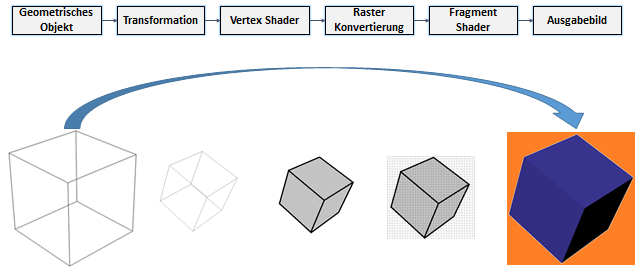
\includegraphics[width=.9\linewidth]{Assets/Computergrafik_Grafik-Pipeline}
  \end{center}
  \begin{itemize*}
    \item algorithmisches Konzept, sowie Realisierung der Grafikkartenhardware ist vergleichbar mit Fließband
    \item spezialisierte Arbeitsstationen (Spezialprozessoren)
    \item jedes geometrische Objekt durchläuft Arbeitsstationen sequenziell
    \item Arbeitsschritte können dadurch gleichzeitig auf verschiedenen Daten ausgeführt werden
  \end{itemize*}
  
  \subsection{Bestandteile}
  \begin{enumerate*}
    \item Programm API 
    \item Treiber 
    \item Vertex-Verarbeitung 
    \item Primitivenbehandlung 
    \item Rasterisierung \& Interpolation 
    \item Fragment Verarbeitung 
    \item Rasteroperation 
    \item Bildspeicher
  \end{enumerate*}
  
  \subsection{Allgemein}
  \begin{itemize*}
    \item Anwendungsprogramm:
    \begin{itemize*}
      \item läuft auf der CPU,
      \item definiert Daten und Befehlsabfolge,
      \item greift dazu über das Grafik-API (z.B. OpenGL, Direct3D) auf die Grafikkarte zu
    \end{itemize*}
    \item Treiber: übersetzt die Grafikbefehle des Programms in die Maschinensprache der speziellen Grafikhardware (Graphics Processing Unit)
    \item Befehle und Daten werden über den Bus (z.B. PCI-Express) von der CPU auf die GPU übertragen
    \item OpenGL-Pipeline: Abarbeitung der Grafikbefehle auf der GPU
    \item Ausgabe des Bildspeichers auf dem Monitor
    \item Treiber schickt Daten/Befehle an die GPU (z. B. via PCIe -Bus)
    \item Funktionsausführung auf der GPU ist dann abhängig vom aktuellen Zustand
  \end{itemize*}
  
  \paragraph{Abarbeitungsreihenfolge auf der GPU}
  \begin{itemize*}
    \item Empfangen der Vertices in einer geordneten Sequenz
    \item Vertexverarbeitung via Vertex Shader. Jeder Input-Vertex im Datenstrom wird in einen Output-Vertex transformiert und beleuchtet
    \item Primitive culling (Verwerfen wenn nicht sichtbar) und clipping (Abschneiden der Polygone am Rand)
    \item Rasterkonvertierung (Polygon Filling) und Interpolation der Attributwerte (x-Koordinate, 1/z, R, G, B, Texturkoordinaten u/v, ...)
    \item Die Daten jedes Fragmentes (Pixel/Subpixel) wird mit einem Fragment Shader verarbeitet. Zu jedem Fragment gehört eine Anzahl Attribute
    \item Per-Sample Operationen: Blending (Alpha-Blending bei Transparenz), Tiefen- und Stencil- Operationen ...
  \end{itemize*}
  
  \subsection{Vertex-Verarbeitung}
  \begin{description*}
    \item[Transformationen] Modell-Transformation, Kamera-Transformation (Model View Matrix) $\rightarrow$ Matrixmultiplikationen $\rightarrow$ Skalarprodukt
    \item[Beleuchtung] Lichtquellen, diffuses \& spekuläres Material: Lambert, Phong-Modell $\rightarrow$ Skalarprodukt
    \item[Skalarprodukte] (Gleitkomma-Multiplikationen und Additionen) werden durch viele parallele Prozessoren auf der GPU effizient verarbeitet
  \end{description*}
  
  %\subsection{Primitive & Primitivenbehandlung}
  %![Primitive; Quelle Computergrafik Vorlesung 2020/21](Assets/Computergrafik-Renderpipeline-primitive.png)
  
  \subsection{Rasterkonvertierung}
  \begin{itemize*}
    \item Edge Tables bereits erzeugt (Polygonsetup)
    \item Rasterkonvertierung/Interpolation entspricht der Scan- Line-Konvertierung, generiert Pixel (Fragments)
    \item Interpolation der x-Werte der Kanten (left/right edge scan)
    \item pro Scan Line: inkrementiere x-Wert (left/right edge)
    \item lineare Interpolation weiterer Attribute
    \begin{itemize*}
      \item $z (1/z)$-Werte,
      \item RGB-Werte (Gouraud Shading),
      \item Texturkoordinaten u/v (affines Texturmapping),
      \item Normalen (Phong Shading)
    \end{itemize*}
    \item sehr wenige Ganzzahloperationen pro Pixel/Bildzeile
    \item Ausnahme z.B. perspektivische TM (FP-Division)
  \end{itemize*}
  
  \subsection{Fragment-Verarbeitung}
  \begin{itemize*}
    \item Weiterverarbeitung auf Basis der interpolierten Attribute im Fragment Shader
    \item Beispiel Phong-Shading: Berechnung des Phong-Beleuchtungsmodells auf Basis der vorher linear interpolierten Fragmentnormalen, -position und Materialdaten sowie der Daten der Lichtquellen und Kameraposition
  \end{itemize*}
  
  \subsection{Rasteroperationen}
  \begin{itemize*}
    \item Abschließende Auswahl/Zusammenfassung der berechneten Fragmentdaten (pro Pixel)
    \item Beispiel: nicht transparente Objekte, Übernahme der Farbwerte mit z-Position, welche am dichtesten an der Kamera ist
    \item Beispiel: transparente Objekte, lineares Blending zwischen schon existierenden Farbwerten und neuesten entsprechend der Transparenz
  \end{itemize*}
  
  \subsection{Performance}
  Einfaches Modell zur Bestimmung der Rechenzeit T:
  $$T = a * \text{Anzahl Vertices} + b * \text{Anzahl Bildpixel}$$
  (a = Aufwand pro Vertex, b = Aufwand pro Pixel)
  
  \begin{itemize*}
    \item Grafikkarten geben ihre Performance an in:
    \begin{itemize*}
      \item Anzahl Polygone / Sekunde (Polygone mit kleiner Pixelanzahl)
      \item Anzahl verarbeitete Pixel / Sekunde
    \end{itemize*}
    \item Problem der Grafik-Pipeline: Langsamste Operation hält Pipeline auf (bestimmt Durchsatz) 
    \item $\rightarrow$ Zwei extreme Situationen:
    \begin{description*}
      \item[Vertex-limited] viele Vertices, kleine Polygone (wenige Pixel), einfache lineare Interpolation der Vertex-Attribute pro Fragment (kleines b )
      \item[Fill rate limited] anspruchsvolle Fragment-Shader (großes b), weniger dafür große Polygone (viele Pixel)
    \end{description*}
    \item Außerdem: Grafikspeicher-Zugriffe sind teuer (Latenz und Bandbreite beachten) z.B. Auslesen gerenderter Bilder aus dem Grafikspeicher
    \item Eine für die Grafikkarte angegebene Performance ist nur unter unrealistisch günstigen Bedingungen zu erreichen.
    \begin{itemize*}
      \item wegen Speicherbandbreite für Vertexzugriffe
      \item da Framebuffer-Reset teuer
      \item Herstellerangaben nur für optimalen Bedingungen
      \item realistisch $\rightarrow\approx 10\%$ der Peak Performance!
    \end{itemize*}
  \end{itemize*}
  
  $$\text{Durchsatz (fps)} \approx \text{Konst.} / \text{Polygonanzahl}$$
  \begin{itemize*}
    \item unter realitischem Durchsatz: Begrenzung durch Bildspeicher
    \item über realisitschem Durchsatz: Begrenzung durch Geometriespeicher
  \end{itemize*}
  \begin{center}
    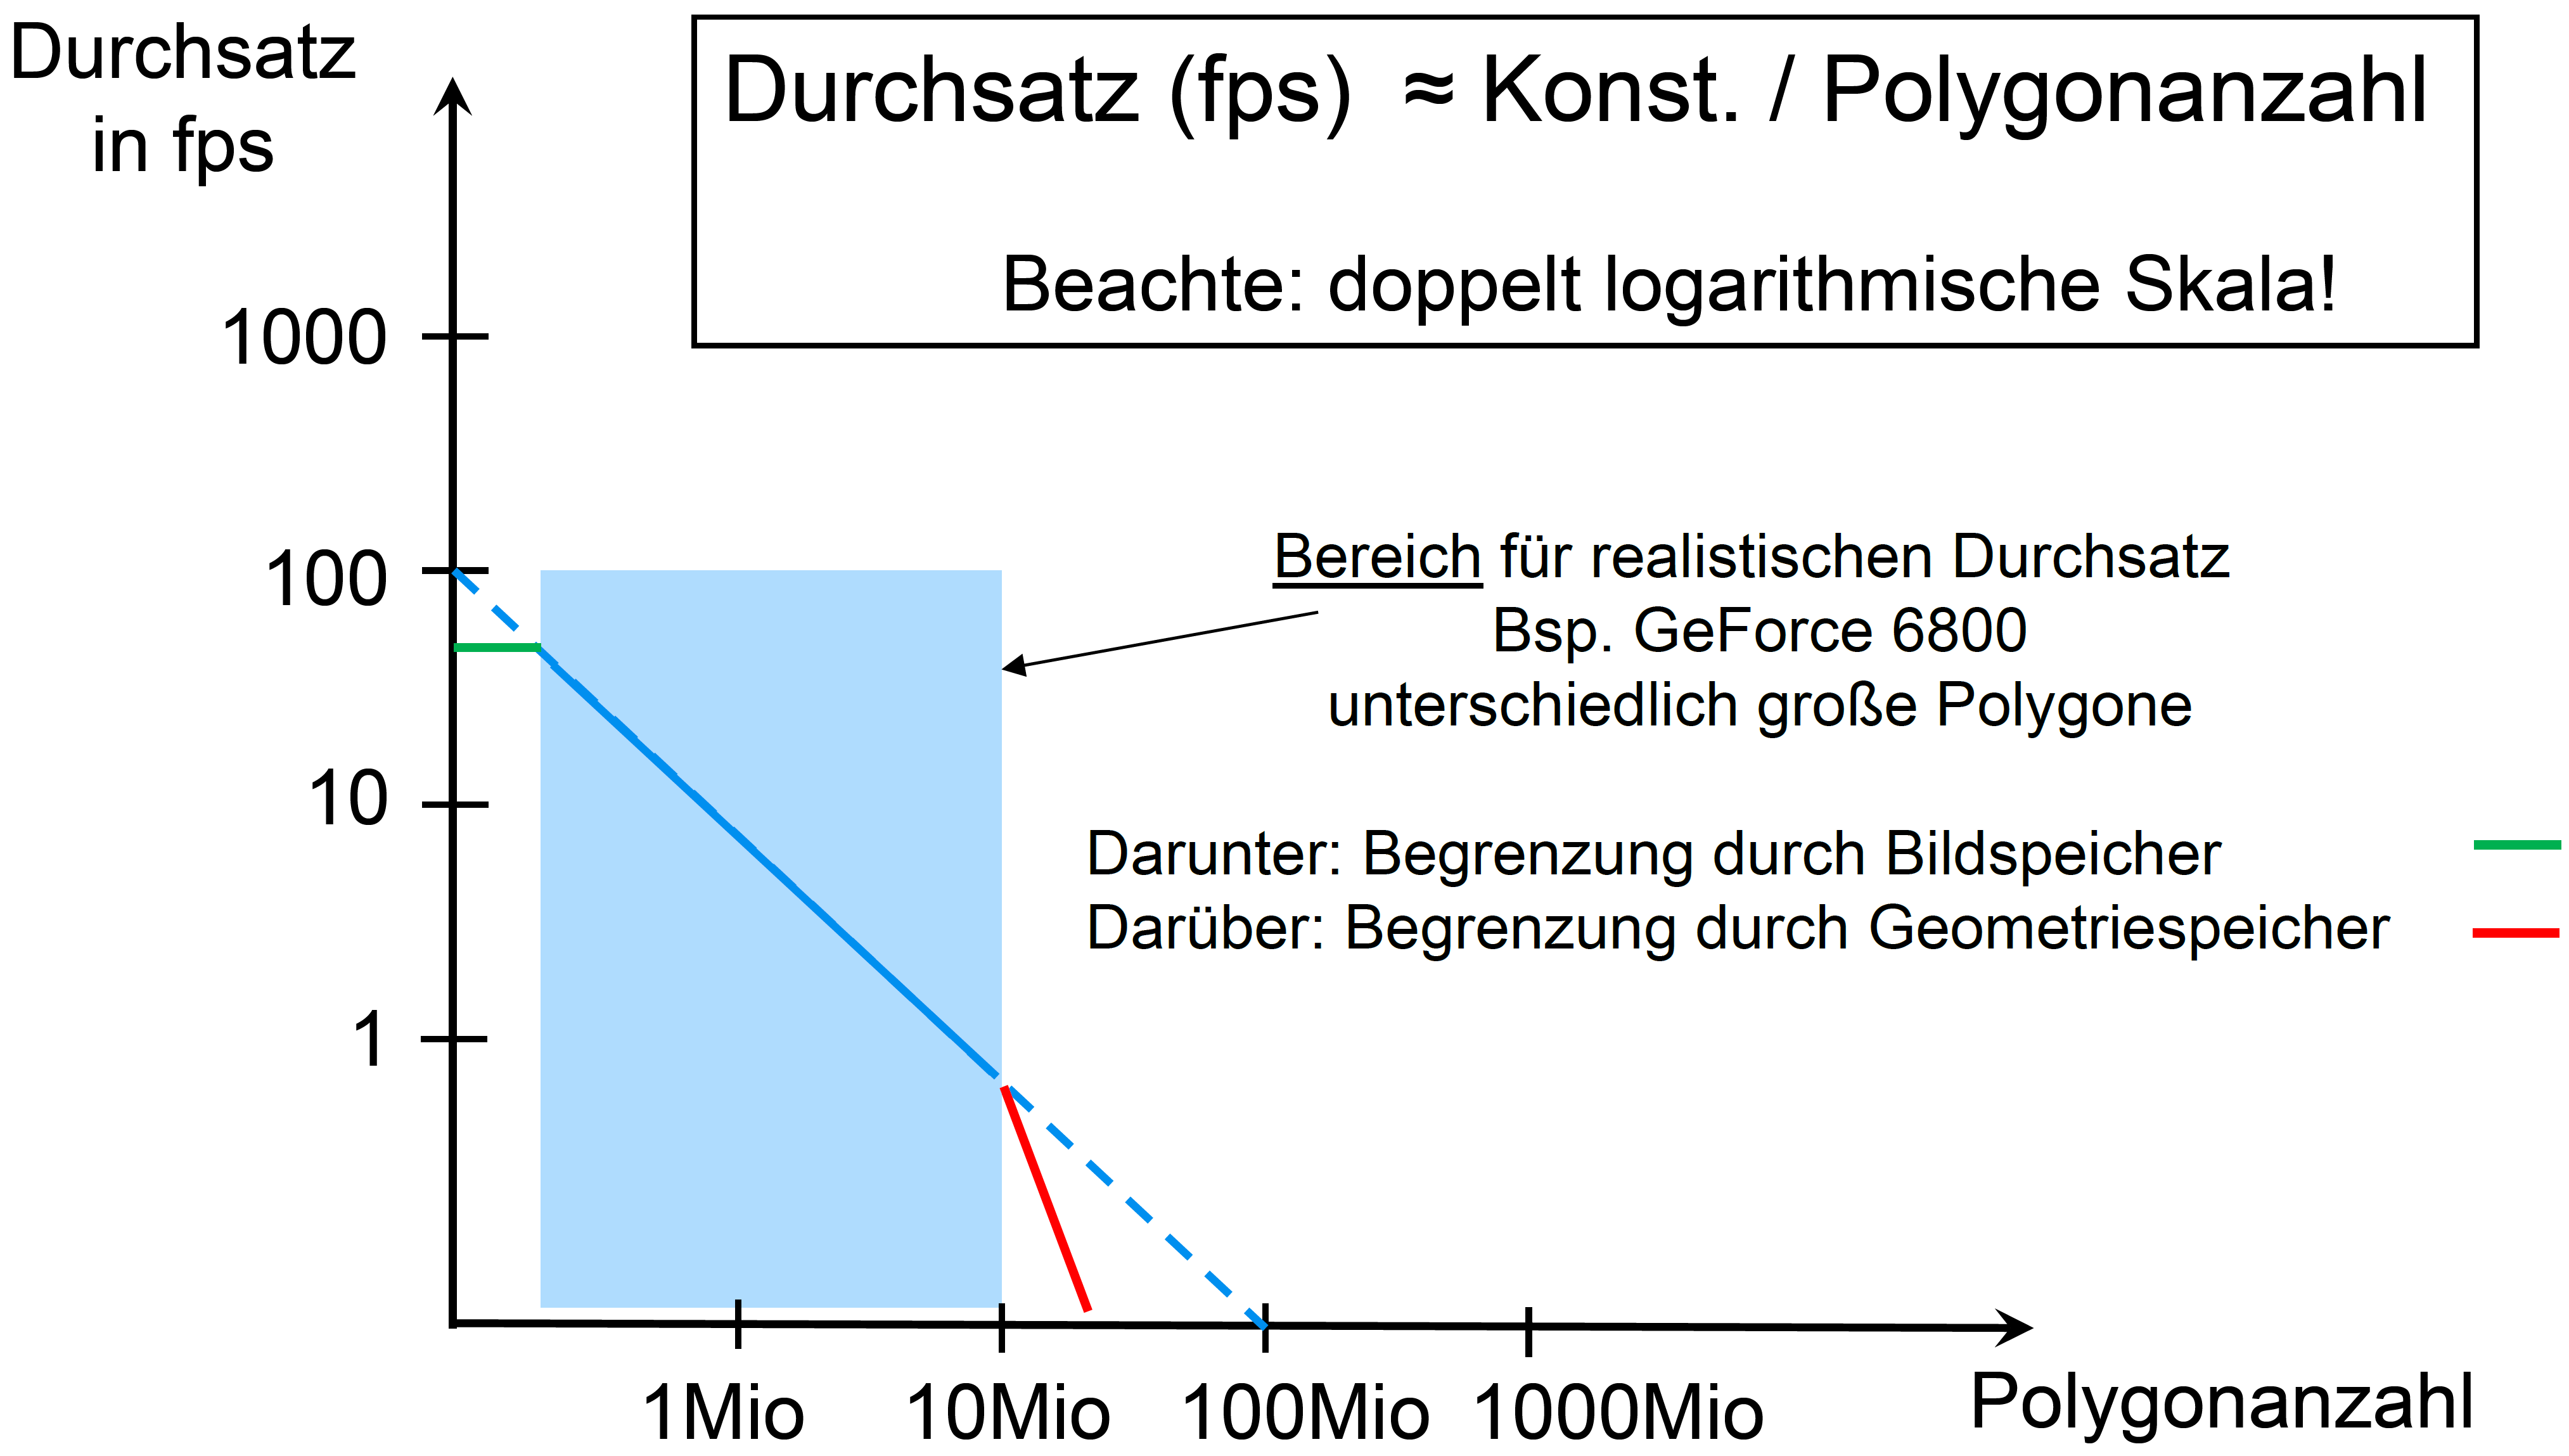
\includegraphics[width=.9\linewidth]{Assets/Computergrafik_GPU-Performance}
  \end{center}
  
  \paragraph{Hardware-Architektur}
  \begin{center}
    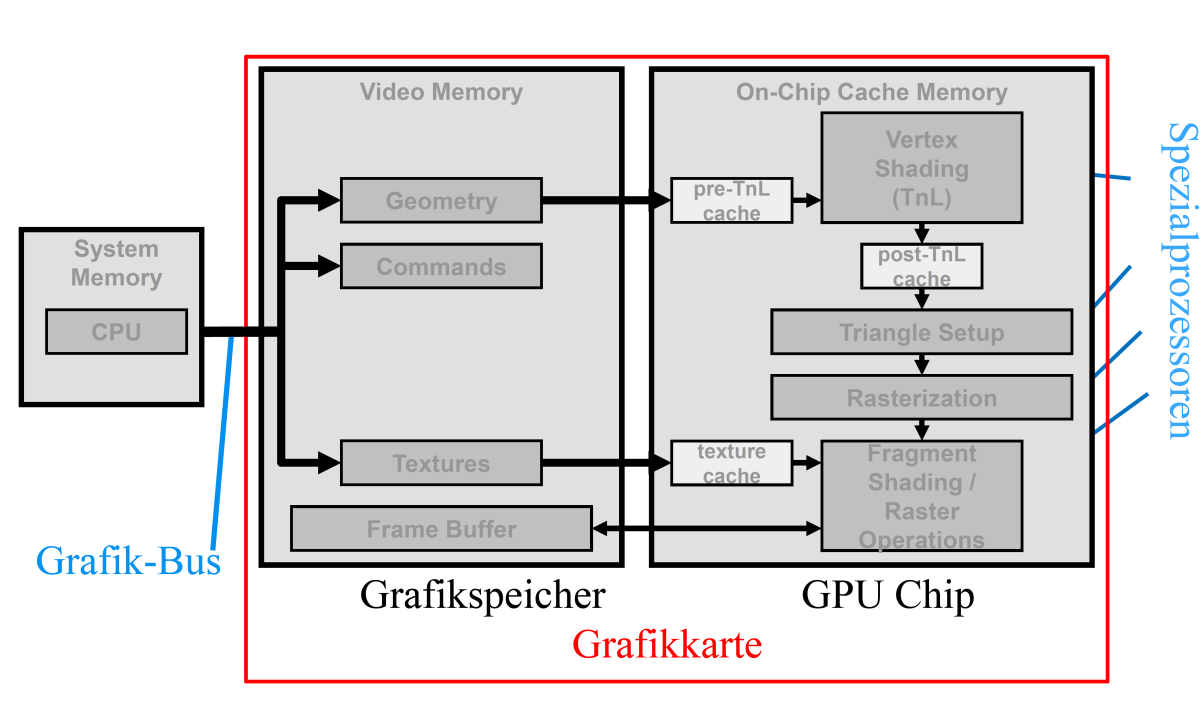
\includegraphics[width=.9\linewidth]{Assets/Computergrafik_GPU_Hardware}
  \end{center}
  
\end{multicols}
\newpage
\begin{multicols}{3}
  \section{Bildverarbeitung}
  \subsection{Operationen auf dem Bildraster}
  Problem der Vorwärtstransformation:
  \begin{itemize*}
    \item Farbwerte sitzen im Zielbild an nicht ganzzahligen Koordinaten, das Ausgabegerät benötigt aber Farbwerte in einem Raster (ganzzahlige Koordinaten)
    \item durch Runden können Löcher im Bild entstehen, einige Pixel werden u. U. mehrfach belegt
  \end{itemize*}
  %![Bildraster Skalieren](Assets/Computergrafik_Bildraster_skalieren.png)
  
  \paragraph{Inverse Transformation}
  \begin{itemize*}
    \item da jedes Pixel im Zielbild B an Position (k,l) Ausgangspunkt der Rechnung ist, bleibt keines unbelegt
    \item keine Löcher mehr
    \item Problem: Auch das Quellbild A ist nur an ganzzahligen Rasterpunkten i,j gegeben. Wie ermittelt man A(x,y) aus den Pixeln A(i,j) im Umfeld von x,y? Wie groß muss das Umfeld sein? $\rightarrow$ Resamplingproblem (Wiederabtastung)
  \end{itemize*}
  
  \paragraph{Rückwärtstransformation der Pixelkoordinaten}
  \begin{itemize*}
    \item Inverse Transformation der Koordination vom Zielbild + Sampling im Originalbild
    \item Es entstehen keine Lücken im Zielbild aber durch Rundung nichtganzzahliger Pixelkoordinaten auf den nächstenganzzahligen Wert können Aliasing-Artefakte entstehen $B(k.l)=A(h^{-1}(k,l))$
    \begin{itemize*}
      \item einzelne Pixel im Originalbild werden öfter gesampelt
      \item einige Pixel im Originalbild werden ausgelassen
    \end{itemize*}
  \end{itemize*}
  %![Rücktransformation I](Assets/Computergrafik_Rückwärtstransformation_Pixelkoordinaten.png)
  
  Rückwärtstransformation der Pixelkoordinaten mit Interpolation benachbarter Pixel:
  \begin{itemize*}
    \item Inverse Transformation der Koordination vom Zielbild + Sampling im Originalbild
    \item bei nicht ganzzahligen Pixelkoordinaten kann man zwischen den benachbarten Pixelwerten im Originalbild interpolieren
    \item dadurch werden die scharfen Flächengrenzen unscharf
    \item aber die wahrgenommenen Grenzen zwischen schwarzen und weißen Flächen können so zwischen den ganzzahligen Pixelwerten positioniert werden
    \item die empfundene Genauigkeit wird durch Antialiasing sogar erhöht!
  \end{itemize*}
  %![Rückwärtstransformation II](Assets/Computergrafik_Rückwärtstransformation_Interpolation.png)
  
  \paragraph{Verkleinern eines Bildes durch Skalierung}
  \begin{itemize*}
    \item Inverse Transformation der Koordination vom Zielbild + Sampling im Originalbild
    \begin{itemize*}
      \item auch hier entstehen zwar keine Lücken im Zielbild beim Transformieren zusammenhängender Bilder
      \item aber beim Sampeln im Originalbild entstehen Aliasing-Artefakte:
      \item z.B. Auslassen jedes zweiten Pixels im Originalbild $\rightarrow$ Zielbild wird uniform weiß (oder schwarz)
    \end{itemize*}
    \item exakte Lösung wäre nur bei doppelter Auflösung möglich
    \item jedoch Auflösung im Zielbild begrenzt
    \item Näherung durch Sampeln und Interpolation mehrerer Nachbarpixel führt zu möglicher Lösung
  \end{itemize*}
  
  \begin{description*}
    \item[Vorwärtstransformation]
    \begin{itemize*}
      \item gesuchte Farbwerte im Zielbild liegen nicht immer an ganzzahligen Koordinaten
      \item durch Rundung können Lücken im Zielbild entstehen
    \end{itemize*}
    \item[Rückwärtstransformation]
    \begin{itemize*}
      \item es entstehen keine Lücken im Zielbild, dennoch können (Sampling) Artefakte (Aliasing) auftreten
      \item diese Artefakte können durch Interpolation mehrerer Pixel teilweise abmildert werden
    \end{itemize*}
  \end{description*}
  
  \subsection{Frequenzraum}
  Ein Bild ist im zweidimensionalen Ortsraum definiert
  \begin{itemize*}
    \item Farb-/Helligkeitswert als Funktion des Ortes W(x,y)
    \item Bei ortsabhängigen Signalen ist mit Frequenz gemeint, nach welcher Distanz (in Pixeln) sich das Muster im Bild wiederholt
    \item Umwandlung von Ortsraum in Frequenzraum durch Fourier-Transformation
    \begin{itemize*}
      \item Bild im Frequenzraum f definiert
      \item $S(f)$ wird Spektrum genannt
    \end{itemize*}
  \end{itemize*}
  %![Frequenzraum](Assets/Computergrafik_Frequenzraum_Signal.png)
  
  Beispiel: 2D-Spektrum eines Schachbrettmusters
  \begin{itemize*}
    \item Kleinstes auf einem Pixelraster darstellbares Muster hat Durchmesser von 2 Pixel
    \item Höchste darstellbare Frequenz $f_x = f_y = 0,5 \text{ Pixel}^{-1}$
    \item Diese Frequenz nennt man Nyquist-Frequenz
  \end{itemize*}
  
  Bildraster als P-dimensionaler Vektorraum:
  \begin{itemize*}
    \item diskrete Grauwertbild $F (i* \delta x, j * \delta y )$ habe M Spalten und N Zeilen
    \item $P = M * N$ ist damit die Dimension des Primärdatenraumes des Bildes
    \item $M * N$ Basisbildern der Dimension $M * N$, jeweils nur ein Pixel den Wert 1 (weiß)
    \item Basisbilder sind damit alle orthonormal
    \item ergeben in grauwertgewichteten Summe das diskrete Bild F
  \end{itemize*}
  %![Frequenzraum II](Assets/Computergrafik_Frequenzraum_diskretes_Bild.png)
  
  Vektoroperationen im Bildraum
  \begin{itemize*}
    \item Skalarprodukte zwischen zwei Bildern
    \item Basistransformation: Ganze Bilder dienen als Basis eines transformierten Bildraumes
    \item Die neuen Basisvektoren müssen linear unanhängig sein und idealerweise orthonormal zueinander stehen
    \item Eine Basistransformation entspricht einer Drehung des Vektorraumes um den Nullpunkt
  \end{itemize*}
  
  \paragraph{Transformation}
  \begin{itemize*}
    %\item Jedes Pixel im gedrehten Raum entspricht einem Bild im Ursprungs-Raum.
    \item Jedes Bild ist Linearkombination der Basisvektoren, entspricht gewichteter Addition von Bildern im Ursprungsraum
    %![Transformation](Assets/Computergrafik_Frequenzraum_Transformation.png)
    \item 4 neue Basisvektoren $B_i$ (2 x 2 Pixel) für unterschiedliche Frequenzen
    %![Basisvektoren](Assets/Computergrafik_Transformation_Basisvektoren.png)
    %(Weiß=+1; Schwarz=-1; Grau=0)
    \item Die 4 Basisvektoren stehen orthonormal zueinander. Test mittels paarweisen Skalar-produkten: $B_iB_k=\begin{cases}1 \text{ falls } i=k\\ 0 \text{ sonst }\end{cases}$
    \item Jedes einzelne Pixel aber auch jedes Bild kann als Linearkombination aus 4 Basisvektoren $B_1$ bis $B_4$ konstruiert werden: $P=a*B_1+b*B_2+c*B_3+d*B_4$
    \begin{itemize*}
      \item Gleichungssystem: 4 Gleichungen für a,b,c,d
      \item Berechnung der Frequenzanteile a bis d über Gleichungssystems $a=P*B_1$
    \end{itemize*}
    %![Basisvektoren II](Assets/Computergrafik_Basisvektor_Linearkombination.png)
  \end{itemize*}
  
  \paragraph{DCT - Discrete Cosinus Transformation}
  \begin{itemize*}
    \item Spezielle Basistransformation: Cosinus Transformation
    \item Jedes Pixel im Cosinus Raum entspricht einem Bild mit Cosinus-Funktionen verschiedener Frequenzen oder Phasen
    \begin{itemize*}
      \item Links oben: Frequenz = Null (Durchschnittswert)
      \item Rechts unten: Anteil der höchsten Frequenz
    \end{itemize*}
    \item Cosinus Raum bildet ein Orthonormalsystem
    \item ein Pixelbild im Ursprungsraum lässt sich zusammensetzen als gewichtete Addition von Bildern mit unterschiedlichen Frequenzen $\rightarrow$ Spektralzerlegung
    \item Ähnlich funktioniert die Fouriertransformation (Sinus und Cosinustransformation)
  \end{itemize*}
  %![DCT](Assets/Computergrafik_DCT.png)
  
  \paragraph{Fouriertransformation}
  \begin{itemize*}
    \item jede periodische Funktion lässt sich darstellen als Summe von $\sin$ und $\cos$ Funktionen
    \item Transformation: stellt Funktion nur anders dar; umkehrbar
    \item Hochpassfilter: ausblenden der tiefen Frequenzen
    %![Hochpassfilter](Assets/Computergrafik_Fourier_Hochpass.png)
    \item Tiefpassfilter: ausblenden der hohen Frequenzen
    %![Tiefpassfilter](Assets/Computergrafik_Fourier_Tiefpass.png)
  \end{itemize*}
  
  \paragraph{Signalrekonstruktion}
  \begin{itemize*}
    \item Abtastfrequenz viel höher als Signalfrequenz im Original
    \item Signalfrequenz liegt unter halber Abtastfrequenz, der Nyquistfrequenz
    \item Samplingtheorem von Nyquist
    \begin{itemize*}
      \item Signale unterhalb der Nyquistfrequenz können rekonstruiert werden
      \item Signale oberhalb der Nyquistfrequenz können nicht rekonstruiert werden
      \item Aliasing-Effekt
    \end{itemize*}
  \end{itemize*}
  
  \paragraph{Anitaliasing}
  \begin{itemize*}
    \item Aliasing bei Bildern entsteht u.a. wenn das Bild in Bezug auf das Abtastraster zu hohe Frequenzen enthält
    \item die höchste zulässige Frequenz wird als Nyquistfrequenz bezeichnet
    \begin{itemize*}
      \item gleich der halben Abtastfrequenz $K_{x,Nyqu}=\frac{1}{2*\delta x}$, $x = Pixelabstand$
      %\item zum besseren Verständnis des Grundproblems noch mal drei Beispiele nebeneinander:
      %![Beispiel](Assets/Computergrafik_Antialiasing_Nyquist.png)
      \item Nachträgliches Filtern kann Aliasing nicht beseitigen
    \end{itemize*}
    \item Rekonstruktion eines Signals mittels Interpolation durch Erzeugen weiterer Samples zwischen den gemessenen Samples (Supersampling)
    \item Dennoch entsteht ein etwas gestörtes Signal $\rightarrow$ abgemilderte Aliasing
    \item bei Rückwärtstransformation ist Samplingrate durch Zielbild bestimmt
    \item Bei Verkleinerung um ein Faktor 2 ist die Samplingrate im Originalbild nur halb so groß wie die Nyquistfrequenz des Originalbildes!
    \item Der Begriff der Nyquistfrequenz erklärt das bekannte Phänomen und verweist auf mögliche Lösungen
    \item Aliasing kann bei der Ausgabe von Graphiken oder Bildinhalten auf Ausgabegeräten entstehen, denn dieser Prozess ist in der Regel mit einer Rasterung (Rasterisation) verbunden
    \item Aliasing entsteht insbesondere dann, wenn die Originale in viel höherer Auflösung vorliegen als das Raster des Ausgabegerätes
    \item Aliasing kann auch bei digitalen Fotografien von kleinteiligen (analogen) Mustern entstehen
    \item Da sich Aliasing-Artefakte nicht nachträglich beseitigen lassen, kann Anti-Aliasing nicht erst dann ansetzen, wenn das Bild bereits fertig gerendert ist
    \item Tiefpassfilterung muss deshalb immer vor dem Resampling angewendet werden
  \end{itemize*}
  
  \subsection{Tiefpassfilter}
  Um Bild korrekt rekonstruieren zu können, muss zuerst im Originalbild die hohen Frequenzen, die oberhalb der Nyquistfrequenz des Zielbildes liegen, eliminiert werden.
  \begin{itemize*}
    \item Zuerst im Originalbild hohe Frequenzen, die oberhalb der Samplingrate des Zielbildes liegen, eliminieren
    \item Danach Sampling des gefilterten Originalbildes durch inverse Transformation jedes Pixels im Zielbild
    \item Die höchsten Frequenzen des Originalbildes können aufgrund der zu geringen Auflösung im Zielbild nicht dargestellt werden.
    \item Reihenfolge wichtig: Wenn man zuerst sampelt und dann das Zielbild filtert, lässt sich u.U. die Originalinformation nicht mehr rekonstruieren
  \end{itemize*}
  
  \subsection{Rekonstruktionsfilter}
  \begin{itemize*}
    \item Nach Eliminierung der hohen Frequenzen ist die Rücktransformation erforderlich.
    \item selbe Ergebnis einfacher, indem die Filterfunktion vom Frequenzraum in den Ortsraum transformiert und direkt im Ortsraum angewendet wird
    \item Box-Filter = ideales Tiefpass-Filter in Frequenzraum; eliminiert alle Frequenzen oberhalb
    \item Box-Filter im FR = sinc-Funktion im Ortsraum $sinc(x)=\frac{sin(x)}{x}$
  \end{itemize*}
  
  Rekonstruktion von Zwischenpixelwerten durch Interpolation benachbarter Pixel
  \begin{itemize*}
    \item Inverse Transformation der Koordination vom Zielbild + Sampling im Originalbild
    \item Bei einer Vergrößerung findet hierbei eine Überabtastung statt
    \item Zur genauen Rekonstruktion von Zwischenwerten kann man interpolieren
    \item Dadurch werden die scharfen unscharf aber die wahrgenommene Genauigkeit nimmt zu $\rightarrow$ Antialiasing
    \item Zur Gewichtung können ebenfalls Filterfunktionen im Ortsraum verwendet werden 
    \item Cut-off-Frequenz = Nyquistfrequenz im Originalbild
  \end{itemize*}
  
  \paragraph{Exakte Interpolation}
  Rekonstruktionsfilter (supersampling) per Sinc-Funktion (Exakte Interpolation):
  \begin{itemize*}
    \item Inverse Transformation: $B(k, l) = A(h^{-1} \{k, l\}) = A(x, y )$
    \item Interpolationsansatz 1 für das Resampling:
    \begin{itemize*}
      \item gewichtete Überlagerung der Abtastwerte aus der lokalen Umgebung des Quellbildes
      \item Gewichte werden durch Interpolationsfunktionen festgelegt
      \item Interpolationsfunktionen bestimmen Qualität des Zielbildes
      \item $A(x,y)=\sum_{i=-\infty}^{\infty}\sum_{j=-\infty}^{\infty}A(i,j) * f_{int}(x-i, y-j)$
      \item Filterkern $f_{int}$ ist zentriert um das Pixel $A(x, y)$
      \item Filter ist selbst auch als Rasterbild definiert
    \end{itemize*}
  \end{itemize*}
  
  Anwendung der Filter auf Bildinformationen: 
  $$G(x,y)=\sum_{m=-size}^{size} \sum_{n=-size}^{size} F(x+m, y+n) * H(m,n)$$
  mit Ausgabebild $G(x,y)$, Eingabebild $F(x+m,y+n)$ und Filterkern $H(m,n)$
  
  Beispiel Filterkern: 5x5 Binominalfilter
  $$H_{5x5}=\frac{1}{256} * \begin{pmatrix} 1\\4\\6\\4\\1\end{pmatrix}\begin{pmatrix}1&4&6&4&1\end{pmatrix}=\frac{1}{256}\begin{pmatrix}1&4&6&4&1\\ 4&16&24&16&4\\ 6&24&36&24&6\\ 4&16&24&16&4\\ 1&4&6&4&1\end{pmatrix}$$
  
  Interpolatiponsansatz 1 / Methode 1: Exakte Interpolation
  \begin{itemize*}
    \item Hinreichend bandbegrenzte Bilder lassen sich theoretisch exakt interpolieren: Multiplikation des Quellbild-spektrum mit Rechtecktiefpass im Frequenzbereich
    \item Im Ortsbereich führt das auf eine diskrete Faltung mit der sinc-Funktion.
    \item In der Theorie gibt es keinerlei Störungen / keine Artefakte.
    \item Praxisproblem: die sinc-Funktion ist unendlich ausgedehnt!
  \end{itemize*}
  
  \begin{description*}
    \item[Sinc Filter]
    \begin{itemize*}
      \item theoretisch ideal (scharfe Grenze) bei gleichmäßiger Abtastung über der Nyquist-Frequenz
      \item besonders bei Kanten starke Ringing-Artefakte 
      \item zur Berechnung des Farbwerts eines Pixels alle Abtastwerte des Bildes herangezogen
      \item einfaches Abschneiden der Sinc-Funktion (Lanczos-Filter) führt zu schlechten Ergebnissen
      \item Ortsraum \& Frequenzraum:
      \begin{center}
        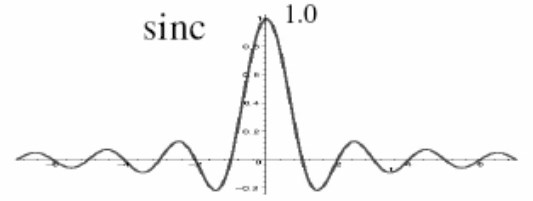
\includegraphics[width=.4\linewidth]{Assets/Computergrafik_Sinc-filter1}
        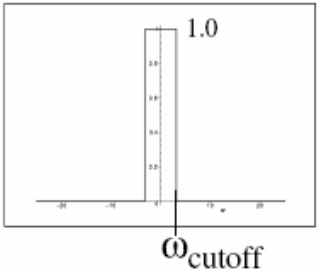
\includegraphics[width=.4\linewidth]{Assets/Computergrafik_Sinc-filter2}
      \end{center}
    \end{itemize*}
    \item[Box-Filter]
    \begin{itemize*}
      \item Alle Abtastwerte innerhalb eines um das Pixel gelegte Quadrat haben die gleiche Gewichtung $\rightarrow$ Mittelwertbildung
      \item allgemein schlechte Ergebnisse, da Fourier-Transformierte eine Sinc-Funktion, die gewünschten Frequenzbereich schlecht isoliert
      \begin{center}
        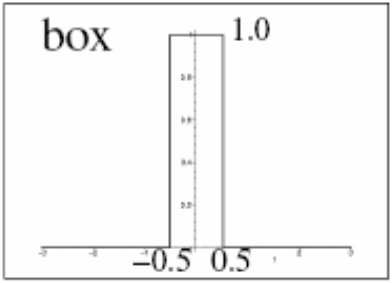
\includegraphics[width=.4\linewidth]{Assets/Computergrafik_Box-filter1}
        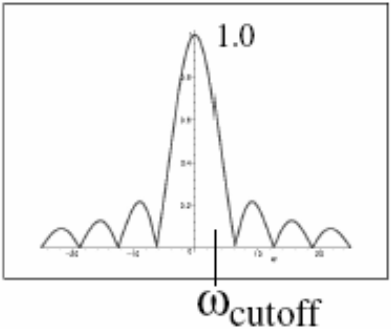
\includegraphics[width=.4\linewidth]{Assets/Computergrafik_Box-filter2}
      \end{center}
    \end{itemize*}
    \item[Kegel-Filter]
    \begin{itemize*}
      \item Gewichtung fällt mit zunehmender Distanz zum Pixel linear ab
      \item etwas bessere Ergebnisse als das Box-Filter
      \item Artefakte sind vorhanden, aber sehr abgeschwächt
      \begin{center}
        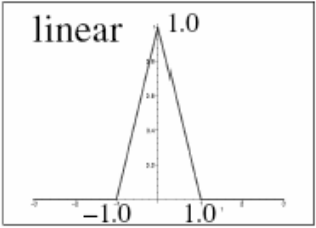
\includegraphics[width=.4\linewidth]{Assets/Computergrafik_Kegel-filter1}
        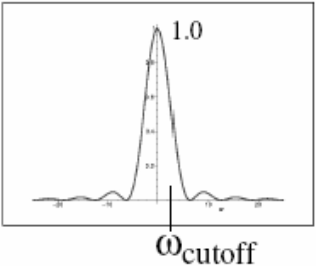
\includegraphics[width=.4\linewidth]{Assets/Computergrafik_Kegel-filter2}
      \end{center}
    \end{itemize*}
    \item[Gauß-Filter]
    \begin{itemize*}
      \item Fouriertransformierte einer Gauß-Funktion ist Gauß-Funktion
      \item Filter führt zu Unschärfe
      \item Aliasing-Effekte sehr gut unterdrückt
      \begin{center}
        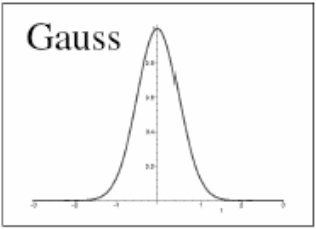
\includegraphics[width=.4\linewidth]{Assets/Computergrafik_Gauss-filter1}
        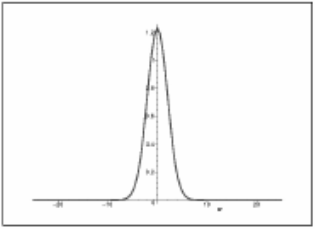
\includegraphics[width=.4\linewidth]{Assets/Computergrafik_Gauss-filter2}
      \end{center}
    \end{itemize*}
    \item[Mitchell-Netravali-Filter]
    \begin{itemize*}
      \item sind stückweise kubische Filter mit vier Pixel breiten Trägern
      \item durch zwei freie Parameter änderbar 
      \item untersuchen aus Rekonstruktionsfiltern resultierenden Artefakte
      \item Bei geeigneter Parameterwahl liefern die Filter einen guten Kompromiss zwischen Unschärfe, Anisotropie und Ringing.
      \item werden auch als bikubische Filter bezeichnet
      \begin{center}
        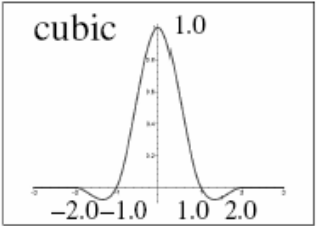
\includegraphics[width=.4\linewidth]{Assets/Computergrafik_Mitchell-Netravali-Filter1}
        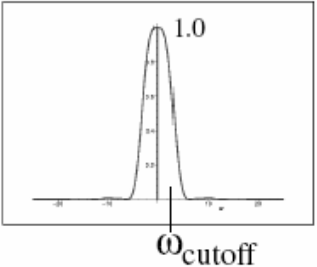
\includegraphics[width=.4\linewidth]{Assets/Computergrafik_Mitchell-Netravali-Filter2}
      \end{center}
    \end{itemize*}
    \item[Nearest Neighbour]
    \begin{itemize*}
      \item einfache Übernahme des geometrisch nächsten Nachbarn aus Quellbild
      \item Entspricht Faltung mit einem Rechteck der Breite $\delta x$ im Ortsbereich, d.h. Multiplikation des periodifizierten Bildspektrums mit einer Sinc-Funktion im Frequenzbereich
      \item Massive Störungen (Artefakte) durch skalierte, z.T. phasengespiegelte Reste von periodifizierten Frequenzanteilen
      \item Verunschärfungen halten sich in Grenzen, da die entsprechende sinc-Funktion bei der Nyquistfrequenz noch nicht wesentlich abgefallen ist
      \item unsymmetrische Operation führt zu frequenzabhängigen, örtlichen Verschiebungen
    \end{itemize*}
    \item[Bilinearer Interpolation]
    \begin{itemize*}
      \item Entspricht der Faltung mit einem Dreieck der Breite $2*\delta x$ im Ortsbereich, d.h. Multiplikation des periodifizierten Bildspektrums mit einer $sinc^2$-Funktion im Frequenzbereich
      \item Reduziertes Aliasing / Artefakte durch schnelleren Abfall der $sinc^2$-Funktion gegenüber sinc
      \item merkliche Verunschärfung durch stärkeren Abfall bei der Nyquistfrequenz
      \item außermittige Interpolation führt zu frequenzabhängigen örtlichen Verschiebungen
    \end{itemize*}
    \item[Sobelgradient] $$H_{xS} =\begin{pmatrix} 1&0&-1\\ 2&0&-2\\ 1&0&-1\end{pmatrix}, H_{yS}=\begin{pmatrix} 1&2&1\\ 0&0&0\\ -1&-2&-1 \end{pmatrix}$$
    \begin{itemize*}
      \item z.B. Kantenextraktion
      \item Differenzbildung (Ableitung) → hohe Frequenzen werden verstärkt!
      \item im Gegensatz dazu sind Tiefpassfilter Integralfilter = gewichtete Summe der Nachbarpixel
    \end{itemize*}
  \end{description*}
  
  
\end{multicols}
\end{document}